\documentclass[modern]{aastex631}
\usepackage{amsmath}
\usepackage{soul}

% Abundance and stellar macros
\newcommand{\mgfe}[0]{[{\rm Mg/Fe}]}
\newcommand{\afe}[0]{[\alpha/{\rm Fe}]}
\newcommand{\femg}{[{\rm Fe}/{\rm Mg}]} 
\newcommand{\xmg}{[{\rm X}/{\rm Mg}]} 
\newcommand{\mgh}{[{\rm Mg}/{\rm H}]}
\newcommand{\feh}[0]{[{\rm Fe/H}]}
\newcommand{\xfe}{[{\rm X}/{\rm Fe}]}
\newcommand{\xh}{[{\rm X}/{\rm H}]}

\newcommand{\logg}{\log(g)}
\newcommand{\teff}{T_{\rm eff}}
\newcommand{\kpc}{\rm \; kpc}
\newcommand{\kel}{\rm \; K}
\newcommand{\msun}{M_{\odot}}
\newcommand{\rgc}{R_{\rm GC}}
\newcommand{\msunvice}{M_{\odot}/M_{\odot \rm formed}}
\newcommand{\MZAMS}{M_{\rm ZAMS}}

\newcommand{\qcc}{q_{{\rm CC,}j}^{Z}}
\newcommand{\qccFe}{q_{{\rm CC, Fe}}^{Z}}
\newcommand{\dqccFe}{dq_{{\rm CC, Fe}}^{Z}/dZ}
\newcommand{\qIa}{q_{{\rm Ia,}j}^{Z}}
\newcommand{\qIaFe}{q_{{\rm Ia,Fe}}^{Z}}
\newcommand{\Acc}{A^{\rm CC}_{i}}
\newcommand{\AIa}{A^{\rm Ia}_{i}}
\newcommand{\fcc}{f_{{\rm CC}, ij}}

\newcommand{\ejg}[1]{\textcolor{red}{EJG says: #1}}
\newcommand{\hogg}[1]{\textcolor{blue}{Hogg says: #1}}

%% Reintroduced the \received and \accepted commands from AASTeX v5.2
%\received{March 1, 2021}
%\revised{April 1, 2021}
%\accepted{\today}

%\submitjournal{ApJ}

% text macros
\newcommand{\name}{\textsl{KPM}} 
\newcommand{\documentname}{\textsl{Article}}

% typesetting stuff
\shorttitle{a data-driven model for nucleosynthesis}
\shortauthors{Griffith \& Hogg}
\addtolength{\topmargin}{-0.4in} % trust the process
\addtolength{\textheight}{0.7in}
\setlength{\parindent}{1.6em}
\renewcommand{\twocolumngrid}{} % trust the process
\renewcommand{\paragraph}[1]{\bigskip\par\noindent{\textbf{#1}}~---}
\sloppy\sloppypar\raggedbottom\frenchspacing % trust the process

%\linespread{1.8}

\graphicspath{{./}{Figures/}}
\begin{document}

\title{\name: A flexible and data-driven $K$-process model for nucleosynthesis}

\correspondingauthor{Emily J. Griffith}
\email{Emily.Griffith-1@colorado.edu}

\author[0000-0001-9345-9977]{Emily J. Griffith}
\altaffiliation{NSF Astronomy and Astrophysics Postdoctoral Fellow}
\affiliation{Center for Astrophysics and Space Astronomy, Department of Astrophysical and Planetary Sciences, University of Colorado, 389~UCB, Boulder,~CO 80309-0389, USA}

\author[0000-0003-2866-9403]{David W. Hogg}
\affiliation{Center for Cosmology and Particle Physics, Department of Physics, New York University, 726~Broadway, New~York,~NY 10003, USA}
\affiliation{Max-Planck-Institut f{\"u}r Astronomie, K{\"o}nigstuhl 17, D-69117 Heidelberg, Germany}
\affiliation{Flatiron Institute, 162 Fifth Avenue, New~York,~NY 10010, USA}

\begin{abstract}\noindent % trust
Stellar surface abundances look like they are produced by two dominant processes, one prompt and one delayed.
We analyze the abundances of 14 elements in [X/Mg] vs. [Mg/H] space for 48,659 stars from APOGEE DR17 with a flexible, data-driven $K$-process model---dubbed \name.
In the fiducial model, where $K=2$, each elemental abundance of each star is described as the vector sum of a prompt (CCSN-like) and delayed (SNIa-like) process.
While prior work derives process vector components from median observed high-Ia and low-Ia abundance trends, we relax these assumptions and simultaneously fit all model parameters to the data, with only minimal constraints to keep the processes interpretable.
We find that our flexible method is able to recover the observed abundance bimodality and that this bimodality is visible to higher [Mg/H] in process amplitude space than in abundance space.
We compare fit parameters and statistics from this new method to those from prior work, finding that the two methods produce similar results, but that \name{} better predicts stellar abundances, especially for C+N and Mn.
We test the validity of the standard two-process model assumptions, such as that Fe is generated by a roughly half-half combination of prompt and delayed sources.
We find that the assumptions of prior works are generally confirmed, but that the inferred fractional contributions from each process are strongly dependent upon Fe assumptions.
We also explore third and fourth processes, calibrated to Ce and Mn, respectively. The additional processes improve the model's ability to predict the stellar abundances, demonstrating the model's ability to extend beyond $K=2$. \name{} enables future research to study the disk's two-dimensionallity, investigate age-abundance label correlations, fit non-bimodal abundance distributions with a multi-component nucleosynthetic model, and much more. \ejg{Add something about code availability.} 
\end{abstract}

\keywords{foo --- bar}
 
\section{Introduction}\label{sec:intro}

After hydrogen, helium, lithium, and beryllium, all other naturally occurring elements are made in the stars, and the collisions of stars.
Stellar surface abundances---the abundances measured by taking a spectrum of a stellar photosphere---are thought to deliver a relatively unprocessed record of the element abundances in the gas from which the star formed \citep[though see e.g.,][]{pinsonneault2001, oh2018, souto2019, vincenzo2021b}.
These birth abundances were set by a combination of nucleosynthetic processes involved in making heavy atomic nuclei, and astrophysical processes involved in delivering atoms from stellar interiors to star-formation sites \citep[e.g.,][]{johnsonja2020}.
Thus nuclear physics and a wide swath of astrophysics are critically intertwined in our understanding of stellar surface abundances, motivating theoretical, experimental, and observational work.

At the present day, stellar surface abundances are not very well explained by \textsl{ab initio}, physics-driven models.
Yields vary from set to set, as they are dependent on progenitor properties and explosion assumptions \citep[e.g.,][]{rybizki2017, griffith2021b}. 
The wide parameter space of progenitor and supernovae models coupled with uncertainties in reaction rates and explosion physics hinder the creation of an accurate nucleosynthetic model from theory alone.
In the long run, it is incumbent upon us to understand these issues and correct the assumptions or calculations underlying our nucleosynthetic and astrophysical models.
In the short run, however, we gather data---tens of millions of abundance measurements on millions of stars in different astronomical surveys such as RAVE, SEGUE, LAMOST, Gaia-ESO, APOGEE/MWM, GALAH, and H3 \citep{steinmetz2006, yanny2009, gilmore2012, desilva2015, luo2015, majewski2017, conroy2019}.
This raises the question: \emph{Can we take a data-driven approach to nucleosynthesis?}

In this \documentname{}, we build a purely data-driven model for the surface element abundances observed in stars.
We treat each star as being a linear combination of nucleosynthetic processes, beginning with one that is primarily responsible for the $\alpha$-element Mg \citep[prompt enrichment, such as core collapse supernovae or CCSN, e.g.,][]{andrews2017}, and one that is primarily \emph{not} responsible for Mg (delayed enrichment, such as Type-Ia supernovae or SNIa).
Beyond these up-front assumption, we try to be agnostic about how the elements are produced.

We build upon the work of \citet[][hereafter G22]{griffith2019, griffith2022} and \citet[][hereafter W19, W22]{weinberg2019, weinberg2022}, who used the bimodality in [Mg/Fe] vs. [Fe/H]\footnote{Where $[{\rm X}/{\rm Y}] = \log({\rm X}/{\rm Y}) - \log({\rm X}/{\rm Y})_{\odot}$ and $({\rm X}/{\rm Y})_{\odot}$ is the solar abundance ratio.} \citep[e.g.,][]{fuhrmann1998, bensby2003, adibekyan2012} to separate stars into populations with high and low SNIa enrichment. Using the median [X/Mg] vs. [Mg/H] abundance trends, these works explain data from the \textsl{GALAH}\footnote{GALAH = GALactic Archaeology with HERMES.} and SDSS-IV \textsl{APOGEE}\footnote{APOGEE = Apache Point Observatory Galactic Evolution Experiment, part of the Sloan Digital Sky Survey} surveys, respectively, with a two-process model. Because the median abundance trends in [X/Mg] vs. [Mg/H] space are largely insensitive to aspects of chemical evolution, such as outflows and variations in star formation history \citep{weinberg2019}, the population abundance trends are set by the nucleosynthetic processes and can be used to empirically constrain Galactic enrichment. 

These works, as well as \citet{ting2022}, find that the Milky Way stellar abundances are well fit two components, down to residuals of 0.01 to 0.02 dex. Simultaneously, \citet{frankel2018} and \citet{ness2022} have found that disk abundances are also well described by a two component model of birth radius and age. Correlations between two-process model parameters and stellar ages and kinematics (W22) suggest that these two 2-dimensional models are somehow interconnected. \ejg{Add bit on why two processes dominate---two main channels v.s. mixing in the disk.}

Beyond standard CCSN and SNIa enrichment many elements have contributions from additional nucleosynthetic processes, such as the rapid ($r$) and slow ($s$) neutron capture processes \citep[e.g.,][]{arlandini1999, bisterzo2014} in asymptotic giant branch (AGB) stars \citep[e.g.,][]{simmerer2004, karakas2016} and merging neutron stars \citep[e.g.,][]{kilpatrick2017}, or atypical supernovae explosion \citep[e.g.,][]{nomoto2013}. After predicting stellar abundances from $\feh$ and $\mgfe$, \citet{ting2022} identify correlated abundance residuals that are unexplained by observational uncertainties, indicative of additional nucleosynthetic processes that standard disk CCSN and SNIa enrichment cannot explain. Results from G22 and W22 support this conclusion, and both works attempt to add additional processes to their models to account for non-CCSN and non-SNIa enrichment, though in a very restrictive manner. Other sources of abundance scatter, such as stochastic sampling of the IMF, IMF variations, and bursty star formation history could also cause deviations away from a two-process model \citep{belokurov2018, griffith2023}.

To date, survey abundances have not been fully exploited to create a data-driven model of nucleosynthesis. While works such as \citet{ting2012}, \citet{casey2019}, and \citet{ratcliffe2022} effectively use clustering algorithms to identify elements with like sources and reduce abundance dimensionality, the results are difficult to translate into a model of nucleosynthesis. Clustering components can be linked to nucleosynthesis sources and enrichment history, but have not yet been be used to describe the enrichment of a single star.

In this work, our main innovations are to relax the assumptions made in G22 and W22, to be more agnostic about the nucleosynthetic processes, and to be more principled with the measurements or inferences from data.
In the $K$ Process Model (\name{}), we find the intersection between reliable facts about nucleosynthesis and good abundance measurements to build an edifice of Galactic enrichment.
The model is hierarchical, in that it learns some parameters (process vectors) that are shared across all stars, but different for each element, and some parameters (process amplitudes) that are shared across all elements, but different for each star.
The parameters output by our model can thus be used as de-noised abundance labels; these will sharpen relationships between abundances and stellar parameters (including birth location and time).

This paper is organized as follows. In Section~\ref{sec:model} we present the assumptions and the implementation of \name{}. In Section~\ref{sec:data} we describe the APOGEE data sample employed in this paper.  We apply \name{} to the APOGEE data in Section~\ref{sec:fiducial} and compare our results to those of W22 in Section~\ref{subsec:w22}. In Section~\ref{sec:variations} we explore variations from the fiducial model, changing our assumptions about Fe production as well as the number of model components. Finally, we discuss and summarize our results in Section~\ref{sec:discussion}.

\section{The $K$-Process Model}\label{sec:model}

As in W22 and G22, we propose that all stellar abundances can be generated by a combination of $K$ nucleosynthetic processes.
In this picture, each element has $K$ metallicity-dependent process vector components that are shared across the full stellar sample, while each star individually has $K$ process amplitudes, which apply across all elements, such that
\begin{equation}\label{eq:mij_k}
    m_{ij} = \log_{10} \, \sum^K_{k=1} A_i^k \, q_{k,j}^Z ~,
\end{equation}
where stars are labeled by $i$ and elements are labeled by $j$.
Each star $i$ has $K$ process amplitudes ($A^k_i$)
and each element $j$ has $K$ process vector components ($q_{k,j}^{Z}$).
The $m_{ij}$ value is the model expected logarithmic abundance of element $j$ in star $i$. In this model, we put forth the following set of assumptions:

\paragraph{1. $K$ processes}
All elements on the periodic table are produced by a combination of nucleosynthetic processes such as CCSN, SNIa, AGB stars, and merging neutron stars \citep{johnsonja2020}. The majority of $\alpha$, light odd-Z, and Fe-peak elements (the elements observed by APOGEE) are dominantly produced by $K=2$ sources, with one being a prompt process or mix of prompt processes, and one being a delayed process or a mix of delayed processes. This is substantiated by theoretical yields \citep[e.g.,][]{anderson2019, rybizki2017} and past successful data-driven models (e.g., G22, W22, \citealp{ting2022}). In this paper we therefore assume that $K \geq 2$, though \name{} could in principle be implemented with $K=1$.

\paragraph{2. Linearity}
At every metallicity, the (linear) $(X/H)$ abundances of a star can be expressed as a linear combination of $K$ processes.
These processes themselves will depend on metallicity, but a linear sum is sufficient to explain all element abundances at any overall metallicity.
Because yields depend on stellar masses and progenitor structure, and because different stars can get to their metallicities by different histories, this assumption must be at least slightly wrong in detail.

\paragraph{3. Non-negativity}
All process vector components for all elements are non-negative and all process amplitudes are non-negative.
This assumption implies that the elements considered here are only produced, and not ever destroyed, by the $K$ processes (relative to hydrogen).
This makes the model similar to a non-negative matrix factorization (\citealt{nnmf} \ejg{Hogg add citation}). In \name{}, this assumption is enforced by requiring that the process vector components and amplitudes are always greater than or equal to zero, such that
\begin{equation} \label{eq:constraint_zero}
    q_{k,j}^Z \geq 0 \; \forall \; Z,k,j \quad \text{and} \quad A_i^k \geq 0 \; \forall \; k,i ~.
\end{equation}

\paragraph{4. Mg production}
All Mg is produced in a prompt process and no other processes contribute to its production.
This is substantiated by theoretical yields where Mg is purely produced by prompt CCSN \citep[e.g.,][]{anderson2019, rybizki2017}.
This assumption (along with non-negativity) breaks a set of symmetries in the process space and makes the processes quasi-interpretable in terms of nucleosynthesis sources.
Because such a prompt process is likely dominated by CCSN \citep[e.g.,][]{andrews2017}, we label the first process with ``CC''. 

In \name{}, this assumption is enforced by fixing the Mg process vector components such that
\begin{equation}\label{eq:qcc_mg_solar}
    q_{{\rm CC, Mg}}^{\,Z_{\odot}} = 1, \quad q_{k>1,{\rm Mg}}^{\,Z_{\odot}} = 0
\end{equation}
at solar metallicity and 
\begin{equation}\label{eq:qcc_mg_z}
    q_{{\rm CC, Mg}}^{\,Z} = q_{{\rm CC, Mg}}^{\,Z_{\odot}}, \quad q_{k>1, {\rm Mg}}^{\,Z} = q_{k>1, {\rm Mg}}^{\,Z_{\odot}}
\end{equation}
at all other metallicities.

\paragraph{5. Fe production}
Fe is produced through a combination of a prompt and delayed process. Because the delayed process is likely dominated by SNIa \citep[e.g.,][]{andrews2017}, we label the delayed process with ``Ia''\footnote{While other enrichment channels with similar timescales may be included in the respective processes, the ``CC'' and ``Ia'' naming convention conforms to the choices in W22 and G22, and avoids the possible confusion of process numbers (1 and 2) with supernovae type (II and Ia).}.
While the prompt process constraint (Mg) is grounded in nucleosynthesis theory, there is no equivalent nucleosynthesis fact to constrain the delayed process.
To break model degeneracies, we also fix the Fe process vector components such that 

\begin{equation}\label{eq:qcc_fe_solar}
    q_{{\rm CC, Fe}}^{\,Z_{\odot}} = 0.4, \quad q_{{\rm Ia, Fe}}^{\,Z_{\odot}} = 1 - q_{{\rm CC, Fe}}^{\,Z_{\odot}} \quad q_{k>2,{\rm Fe}}^{\,Z_{\odot}} = 0
\end{equation}
at solar metallicity and 
\begin{equation}\label{eq:qcc_fe_z}
    q_{{\rm CC, Fe}}^{\,Z} = q_{{\rm CC, Fe}}^{\,Z_{\odot}},  \quad 
    q_{{\rm Ia, Fe}}^{\,Z} = q_{{\rm Ia, Fe}}^{\,Z_{\odot}} \quad 
    q_{k>2, {\rm Fe}}^{\,Z} = q_{k>2, {\rm Fe}}^{\,Z_{\odot}}
\end{equation}
at all other metallicities.
This assumption places a star with purely prompt enrichment on the low-metallicity $\mgfe$ plateau near 0.4 dex, in agreement with APOGEE observations but in contention with recent results from \citet{conroy2022} which places the $\mgfe$ plateau near 0.6 dex.
We explore the impact of different $\qccFe$ assumptions in Section~\ref{subsec:qccFe}.

\paragraph{6. Metallicity dependence}
We permit the process vector components for all elements other than Mg and Fe to float as a function of metallicity.
The variation is parameterized by a linear spline in log-process space, attached to a set of variable control points. We assume that a particular set of hard-coded knots are sufficient to capture the metallicity dependence. \hogg{This could be mentioned in passing in the discussion where you talk about model improvements.}

\paragraph{7. APOGEE abundances and uncertainties}
We assume that the APOGEE abundances and uncertainties can be used for this project.
This is not the same as assuming that they are correct, but rather that it is possible and useful to build an interpretable model to explain them. We describe the potential data systematics in Section~\ref{sec:data}.
The APOGEE errors may be slightly underestimated for some element measurements, so we add a softening parameter $Q$ to inflate the uncertainties on abundance-outlier stars (see Equation~\ref{eq:inflate_ivar}).

\paragraph{8. Robust likelihood function}
The observed value of [X/H] can be described as the $K$ process expectation plus observational noise and/or other sources of intrinsic abundance scatter that are not included in this model:
\begin{equation} \label{eq:xh}
    \xh_{ij} = m_{ij} + \text{noise} ~,
\end{equation}
where $m_{ij}$ is the expectation value given in Equation \ref{eq:mij_k} for star $i$ and element $j$.
The expression in Equation \ref{eq:xh} can be thought of as the key assumption underlying our likelihood function.
In detail the (negative two times the) log likelihood function is given by a chi-squared ($\chi^2$) objective
\begin{equation}
    \chi^2 = \sum_{ij} \, \frac{1}{\sigma_{ij}^2} \, (\xh_{ij} - m_{ij})^2 + Q ~,
\end{equation}
where $1/\sigma_ij^2$ is the (robust; see below) inverse variance on measurement $ij$,
and $Q$ is a light regularization that depends on the parameters.

Because we don't want to be too drawn or influenced by outlier points, we don't use the observed errors $\sigma_{{\rm obs},ij}$ in the likelihood, but instead we soften them in the spirit of iteratively reweighted least squares (HOGG CITE):
\begin{equation}\label{eq:inflate_ivar}
    \frac{1}{\sigma_{ij}^2} = \frac{Q^2/\sigma_{{\rm obs},ij}^2}{Q^2 + (\xh_{ij} - m_{ij})^2 /\sigma_{{\rm obs},ij}^2 },    
\end{equation}
where $Q$ is a softening parameter, which is set to $Q=5$.

\paragraph{9. Implementation and optimization} 
With the above assumptions in place, the likelihood function can be optimized to a set of stellar abundances.
The model is initialized at the Mg and Fe process vector components from Equations~\ref{eq:qcc_mg_solar} --~\ref{eq:qcc_fe_z}. It subsequently optimizes the process amplitudes (dubbed the $A$-step) using only Mg and Fe at fixed process vector components, and then optimizes the process vector components (dubbed the $q$-step) for all elements at fixed process amplitudes.
The $A$-step and $q$-step are alternated, repeating 48 rounds of optimization and updating the best-fit parameters when the objective function improves. We find few differences in the best-fit parameters when we decrease the number of iterations to 32, indicating that the model quickly finds a good solution.  
In detail the optimizations are performed with a nonlinear $\chi^2$ minimization algorithm (Gauss--Newton nonlinear least-squares) from \texttt{jaxopt}\footnote{\url{https://jaxopt.github.io/}}.

\bigskip
\name{} mirrors the two-proccess model from prior work (G22, W22) but, unless otherwise noted, the assumptions weaker, there is a likelihood function in play, and the implementation is more general.
In particular, we don't assume anything about the relationships between the process vector components and the morphologies of observed element-abundance ratio diagrams.

\section{Data}\label{sec:data}

In this paper, we employ stellar abundances from APOGEE DR17 \citep{abdurrouf2022}, part of the SDSS-IV \citep{majewski2017}. The APOGEE survey obtains high-resolution ($R\sim22,500$) near-infrared (IR) observations \citep{wilson2019} for stars in the Galactic disk, halo, bulge, and nearby satellites/streams. Observations are taken with two nearly identical spectrographs on the 2.5m Sloan Foundation telescope \citep{wilson2019} at Apache Point Observatory in New Mexico and the 2.5m du Pont Telescope \citep{bowen1973} at the Las Companas Observatory in Chile. Spectral data are reduced and calibrated with the APOGEE data processing pipeline \citep{nidever2015}, after which stellar parameters and abundances are calculated with ASPCAP \citep[APOGEE Stellar Parameter and Chemical Abundance Pipeline;][]{holtzman2015, garcia2016}. See \citet[][DR16]{jonsson2020} and Holtzman et al. (in prep., DR17) for a more detailed description of APOGEE data reduction and analysis, and \citet{zasowski2013, zasowski2017} and \citet{santana2021} for a discussion of survey targeting.

APOGEE DR17 reports stellar parameters, including $\teff$ and $\logg$, as well as 20 elemental abundances: C, \ion{C}{1}, N, O, Na, Mg, Al, Si, S, K, Ca, \ion{Ti}{1}, \ion{Ti}{2}, V, Cr, Mn, Fe, Co, Ni, and Ce for 657,135 stars. Among these elements and ions, some are measured more precisely than others. We exclude Ti from our analysis as there are large differences between the abundances derived from the \ion{Ti}{1} and \ion{Ti}{2} lines \citep{jonsson2020}. We also exclude P and V, as the P abundances are measured from a few very weak spectra features and V abundances are one of the least precise and least accurate labels \citep{jonsson2020}. Both P and V display strong abundance artifacts and large scatter. Among the remaining elements, we note the following concerns: weak Na spectral features, large abundances scatter in S, significant systematic artifacts in Cr abundances at super-solar metallicities, strong unaccounted for NLTE effects on Mn abundances, and large abundance scatter in Co and Ce---both derived from one line. Further, we note that DR17 is the first time Ce abundances have been included in APOGEE data products. For a more detailed discussion of abundance systematics and their effects on population trends, see \citet{jonsson2020} and \citet{griffith2021a}.

For our stellar sample, we select a subset of APOGEE DR17 stars with the goal of minimizing statistical errors from poor observations and systematic errors from abundance trends with $\teff$ and/or $\logg$ while preserving a sufficient number of stars to conduct a meaningful statistical analysis across the Galactic disk. To remove poor quality data points, we require ASPCAP flags \texttt{STAR\_BAD} and \texttt{NO\_ASPCAP\_RESULT} equal zero. We only include stars from the main survey sample (\texttt{EXTRATARG} = 0), and use named abundances (\texttt{X\_FE}), as recommended by \citet{jonsson2020}. In addition to these quality cuts, we apply the following sample selection:
\begin{itemize}
\itemsep0em
    \item $\mgh > -0.75$
    \item S/N $\geq 200$
    \item $\logg = 1-3$ dex
    \item $\teff = 4000-5200$ K.
\end{itemize}
To eliminate red clump (RC) stars, which show abundance variations from the RGB sample \citep{vincenzo2021a}, we cross-match with and remove stars that appear in the APOGEE RC VAC \citep{bovy2014}. These cuts result in a sample of 48,659 stars.  

We present abundance for Mg, O, Si, S, Ca, C+N, Na, Al, K, Cr, Fe, Ni, Mn, Co, and Ce. In the analysis of each element, X, we drop stars with \texttt{X\_FE\_FLAG} (maximum of $\sim 700$ for Ce). While the surface abundances of C and N differ from the stellar birth abundances for RGB stars due to the CNO processes and dredge-up events \citep{iben1965, shetrone2019}, the total C+N abundance remains constant. As in W22, we consider C+N as an element, taking [(C+N)/H] to be 
\begin{equation}
    [\text{C+N}/\text{H}] = \log_{10}(10^{\text{[C/H]}+8.39} + 10^{\text{[N/H]}+7.78}) - \log_{10}(10^{8.39} + 10^{7.78})
\end{equation}
using logarithmic solar abundances for C (8.39) and N (7.78) from \citet{grevesse2007}. We further adopt the error on the [C/Fe] abundance as the error on [C+N/Fe], since C typically dominates in the abundance ratio.

We plot the distributions of all abundances in [X/Mg] vs. [Mg/H] for our sample in the first column of Figures~\ref{fig:all_param1} and~\ref{fig:all_param2}. 

\begin{figure*}[htb!]
    \centering
    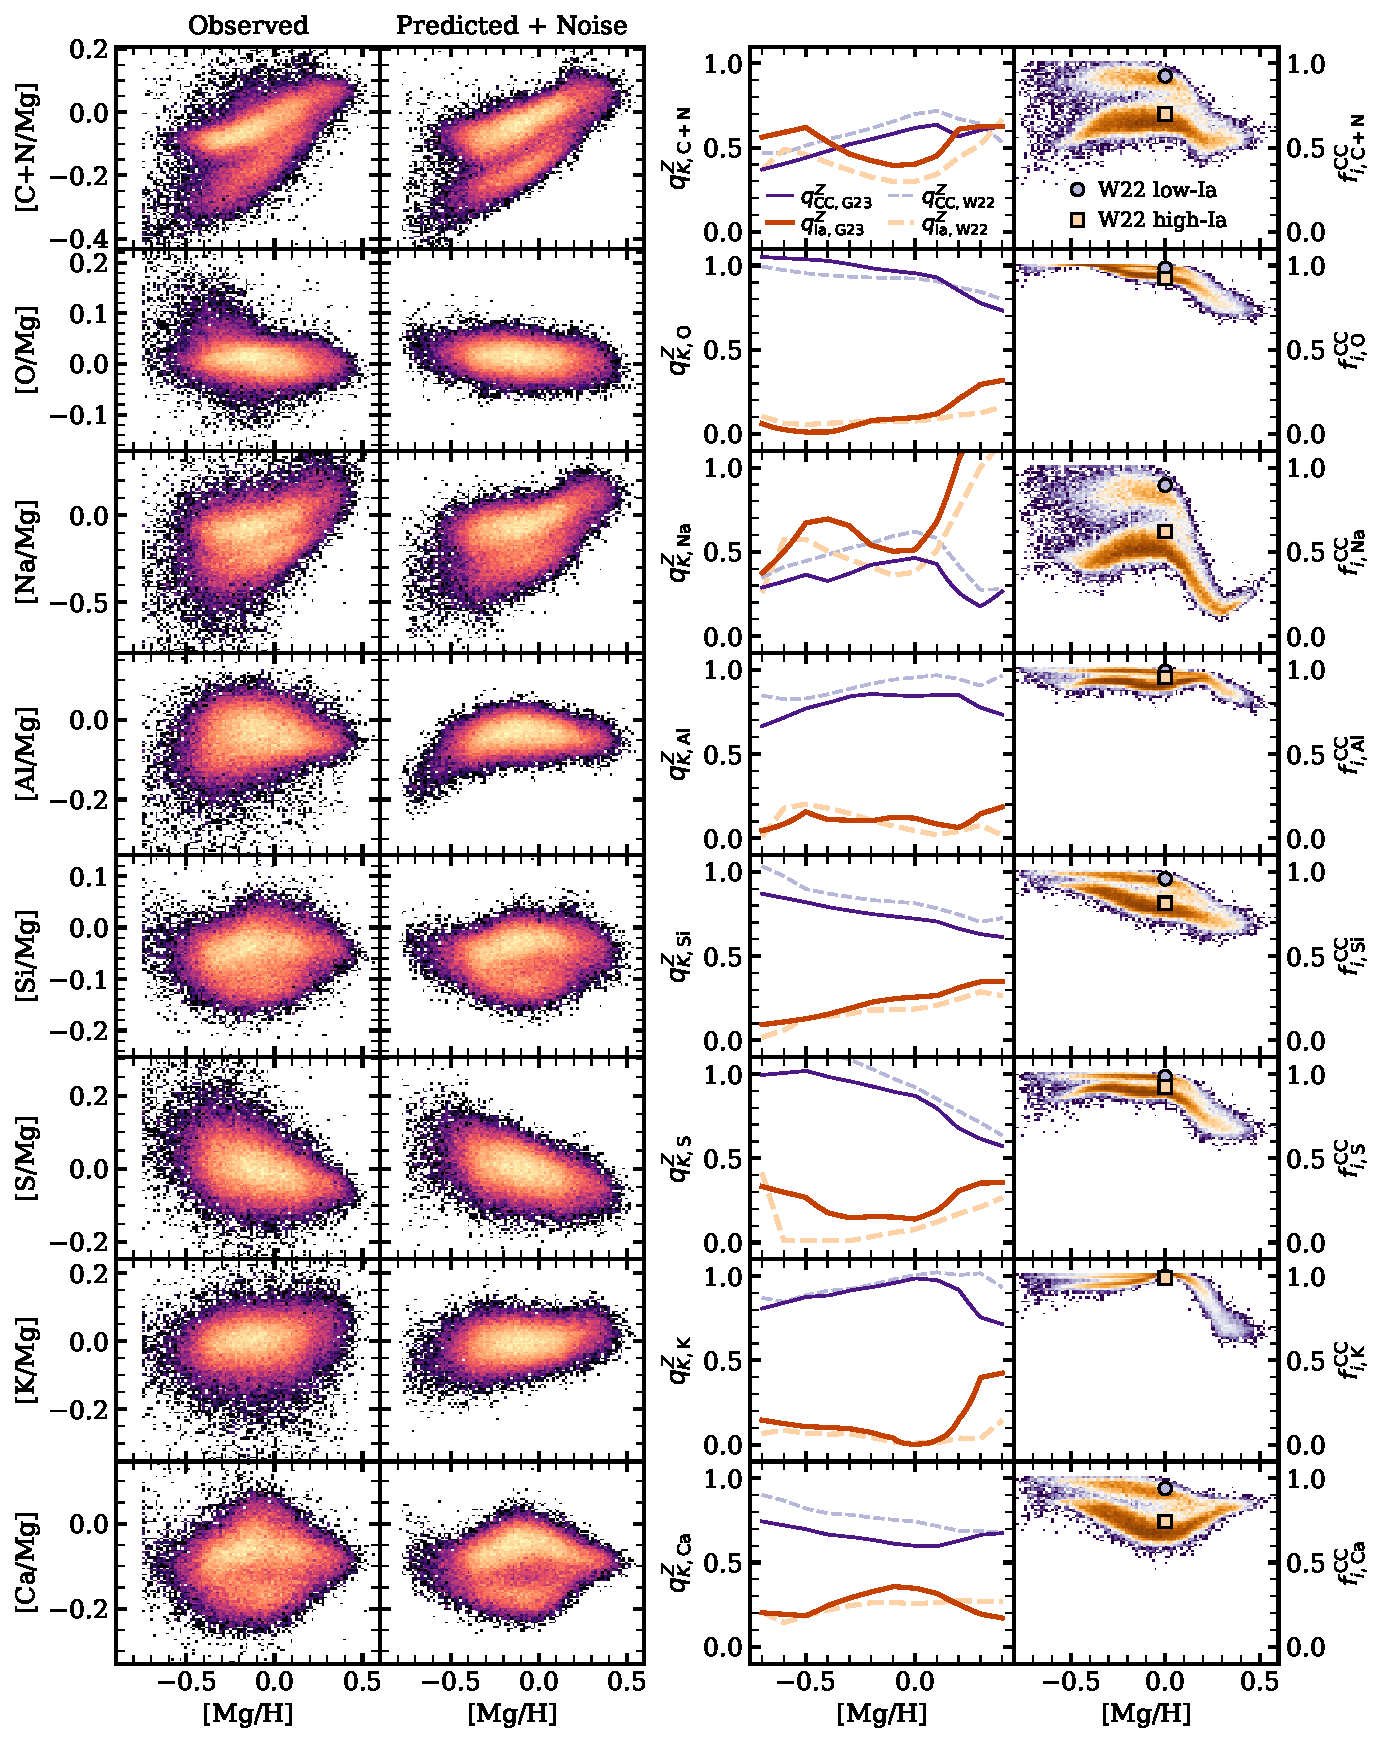
\includegraphics[width=\textwidth]{Paper/Figures/all_param1.pdf}
    \caption{Abundance distributions and \name{} parameters for C+N, $\alpha$, and light odd-$Z$ elements. First column: observed abundance distributions in [X/Mg] vs. [Mg/H]. Second column: The predicted [X/Mg] vs. [Mg/H] abundance distribution of the fiducial plus estimated noise. Third column: process vector components $\qcc$ (purple) and $\qIa$ (orange) from this work (G23, solid, dark lines) and W22 (light, dashed lines). Fourth column: distribution of fractional contribution from the prompt process ($\fcc$) predicted by the fiducial model. We plot the median $\fcc$ values of the low-Ia (orange square) and high-Ia (purple circle) populations in the solar metallicity bin from W22 for comparison.}
    \label{fig:all_param1}
\end{figure*}

\begin{figure*}[htb!]
    \centering
    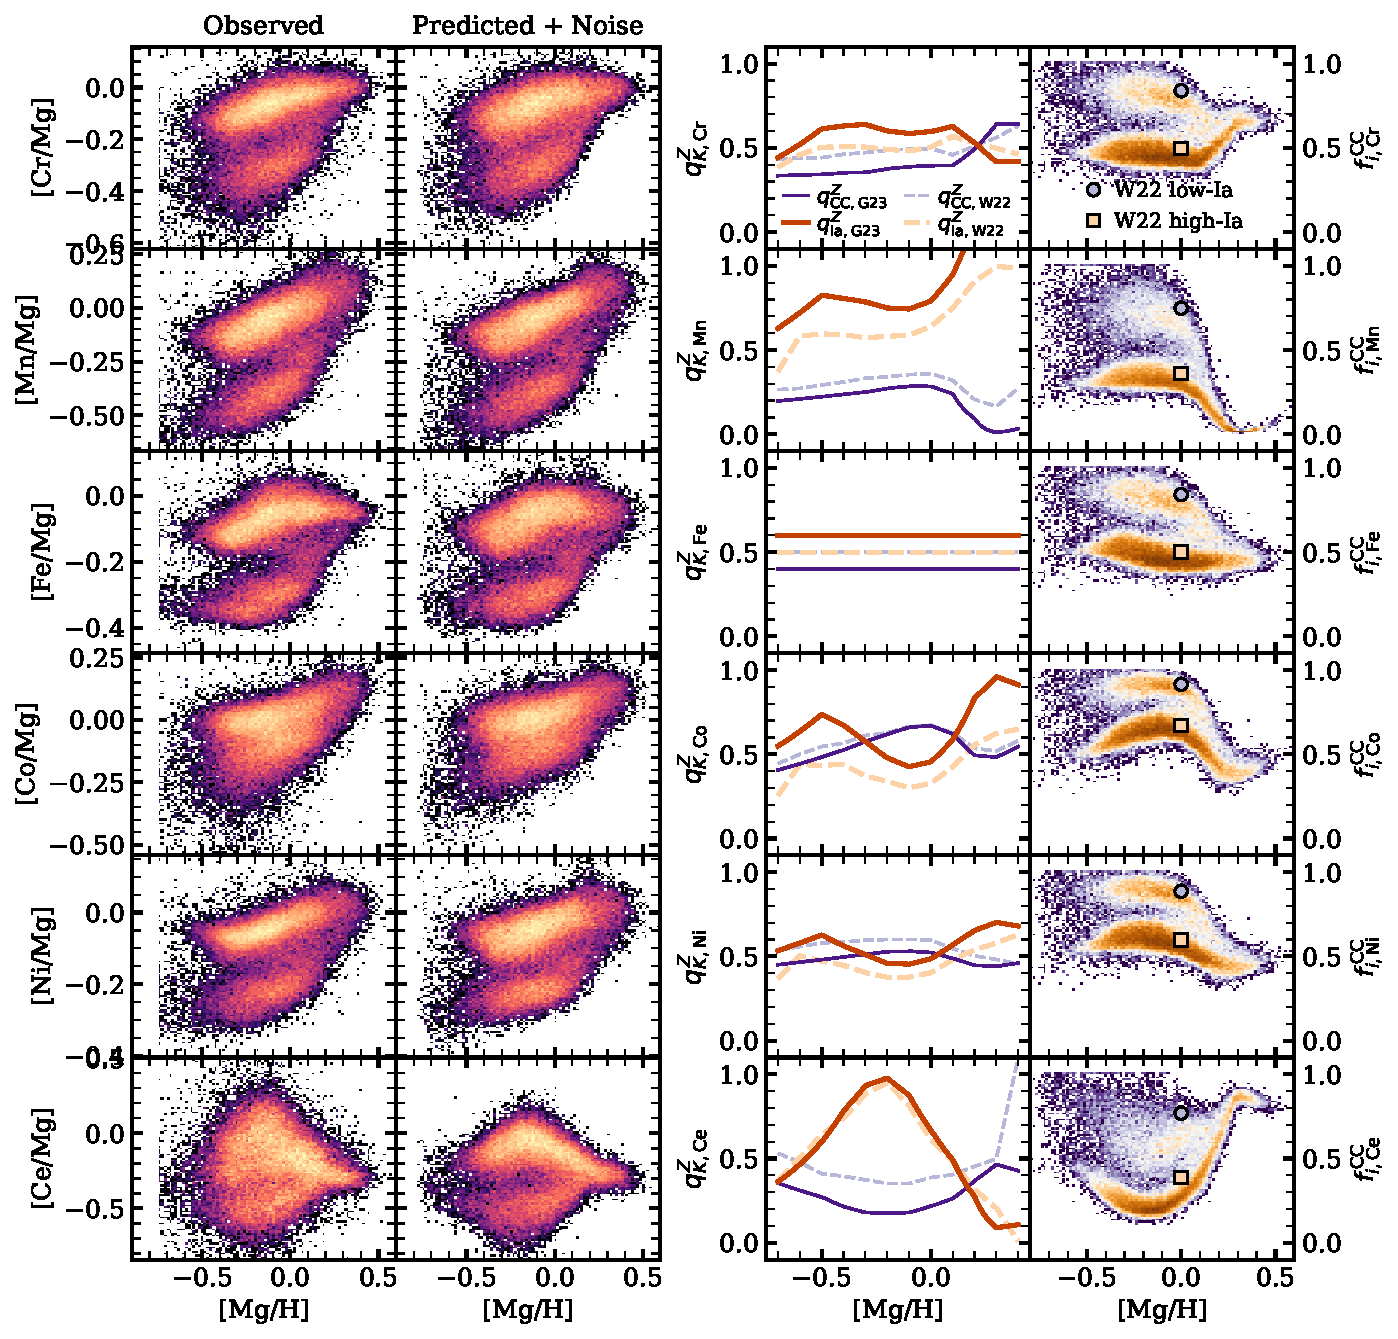
\includegraphics[width=\textwidth]{Paper/Figures/all_param2.pdf}
    \caption{Same as Figure~\ref{fig:all_param1}, but for Fe-peak elements and Ce.}
    \label{fig:all_param2}
\end{figure*}


\section{The Fiducial Model} \label{sec:fiducial}

We fit the APOGEE sample with our fiducial model of $K=2$, such that
\begin{equation}\label{eq:m_ij}
    m_{ij} = \log_{10}(A_i^{\rm CC} \, q_{{\rm CC},j}^Z + A_i^{\rm Ia} \, q_{{\rm Ia},j}^Z)
\end{equation}
with the assumptions from SEction~\ref{sec:model}. This fit produces process vector components $\qcc$ and $\qIa$ as a function of $\mgh$ for each element and process amplitudes $\Acc$ and $\AIa$ for each star. From the model parameters, we can calculate fractional contributions from each process as well as a full suite of predicted $K=2$ process abundances.

\subsection{Process Parameters and Fractional Contributions} \label{subsec:parameters}

We plot the process vector components as a function of $\mgh$ in the third column of Figures~\ref{fig:all_param1} and~\ref{fig:all_param2}. The process vector components inform us about the relative contribution of prompt and delayed processes to the formation of the elements, as well as the metallicity dependence of the enrichment. By definition, $\qccFe=0.4$ at all metallicities. For Fe only, we also require $\qccFe + \qIaFe = 1$, implying $\qIaFe=0.6$. No such constraints are placed on any other element. 

In the fourth column of Figures~\ref{fig:all_param1} and~\ref{fig:all_param2}, we plot the distribution of fractional contributions from the prompt process ($\fcc$) to each element, where
\begin{equation}\label{eq:fcc}
    \fcc = \frac{\Acc \, \qcc}{\Acc \, \qcc + \AIa \, \qIa}.
\end{equation}
We generally find that the distributions are bimodal, like the observed abundance patterns, as the high-Ia and low-Ia populations have differing fractional contributions from prompt and delayed sources.

We find that the $\alpha$-elements (O, Si, S, Ca) are best fit with $\qcc$ and $\fcc > 0.5$ at all metallicities. This is in agreement with theoretical prediction that $\alpha$-elements are dominated by prompt CCSN production \citep[e.g.][]{andrews2017}. O, a Mg-like element theoretically purely produced in prompt CCSN, shows $\fcc$ near 1 from $\mgh=-0.75$ to solar. At supersolar $\mgh$, the delayed process contributes to O production, driving the $\fcc$ value down to $\sim 0.8$ at $\mgh=0.4$. S behaves like O, with almost entirely prompt production up to solar metallicity, after which delayed enrichment contributes more significantly. Conversely, we find that Si and Ca are best fit with prompt and delayed enrichment at all metallicities, though the prompt process always dominates. For Si, the delayed process appear to increase linearly with $\mgh$, while the Ca delayed enrichment increases from $\mgh$ of $-0.75$ to $-0.1$ and then decreases from $\mgh$ of $-0.1$ to $0.5$.

The process vector components of light odd-$Z$ elements Al and K resemble those of the $\alpha$-elements, such as S. Both exhibit $\qcc$ and $\fcc$ near 1 through solar metallicity, with an increase in $\qIa$ and downturn in $\fcc$ at supersolar metallicities (especially for K). The behavior of the Na process vector components is more complex, with peaks and troughs in $\qIa$. We find that Na has the strongest contributions from the delayed process of all $\alpha$ and light odd-$Z$ elements, with $\qIa \gtrsim 0.5$ at almost all values of $\mgh$ and $\fcc < 0.3$ at $\mgh > 0$. The strong delayed contribution to Na is in agreement with findings of W22 and G22, and in tension with theoretical yields \citep[e.g.][]{andrews2017, rybizki2017}.

Unlike $\alpha$ and light odd-$Z$ elements whose delayed production is dominated by SNIa, C and N are thought to be promptly produced in CCSN with additional delayed enrichment from AGB stars \citep[e.g.][]{andrews2017}. We find that the prompt and delayed processes both contribute significantly, and nearly equally, across our stellar sample. Though theoretical N yields from AGB stars have a strong metallicity dependence \citep{karakas2010, ventura2013, cristallo2015, johnson2022}, we observe only a slight positive metallicity dependence in $\qcc$ and a shallow dip in $\qIa$. We find a population of stars with $\fcc$ near 0.9 and a population near 0.4. 

The Fe-peak elements (Cr, Mn, Fe, Co, Ni) are thought to be produced through prompt CCSN production and delayed SNIa production \citep[e.g.][]{andrews2017}. By construction, $\qccFe=0.4$ and $\qIaFe=0.6$ at all metallicities. This produces a bimodal distribution in $\fcc$ similar to that observed in abundances space. Because of our choice of $\qccFe$, only a few stars have $\fcc=1$ (see Section~\ref{subsec:qccFe}). We instead observe a population with $\fcc$ near 0.8 and a population near 0.4. The process vector components and $\fcc$ distribution for Cr and Ni strongly resemble those of Fe. All three elements have even atomic numbers. At supersolar metallicity, we find that the prompt process dominates Cr production, resulting in an upturn in $\fcc$. Conversely, Ni displays a dominant, and increasing, delayed proccess vector component at supersolar metallicities. The process vector components for Mn and Co (odd atomic numbers) show a complex metallicity dependence, more resembling that of Na. Both elements display a strong delayed process, with the Mn $\qIa > 0.5$ at all metallicities and $> 1$ for $\mgh > 0.1$. Mn is the only element for which $\fcc$ decreases to 0 for $\mgh \gtrsim 0.2$. 

Finally, we find that the delayed process dominates Ce production at intermediate metallicity, with $\qIa$ increasing up to $\mgh \approx -0.2$ and then decreasing to nearly 0 at $\mgh \approx 0.3$. The Ce $\fcc$ values are clustered near 0.25 around $\mgh$ of 0.2, then increase such that the abundances are almost entirely dominated by prompt enrichment at high metallicity.

In addition to process vector components, each star is fit with a prompt and delayed process amplitude, $\Acc$ and $\AIa$ respectively. All elemental abundance are used in the calculation of these amplitudes, so they can be interpreted as ``de-noised'' abundance labels. The value of $\Acc$ traces the metallicity (specifically $\mgh$) while the ratio of $\AIa/\Acc$ traces the $\femg$ abundance. In the left panel of Figure~\ref{fig:As} we plot the distribution of $\AIa/\Acc$ vs. $\Acc$. We find a bimodal distribution, similar to the Tinsley-Wallerstein diagram ($\mgfe$ vs. $\feh$, \citealp{wallerstein1962, tinsley1979, tinsley1980}), as was found in W22 and G22. We stress that the presence of the abundance bimodality was not fed into our model, and yet it is recovered in the best-fit process amplitudes. The stars with larger $\AIa/\Acc$ values correspond to the high-Ia population, and those with low $\AIa/\Acc$ correspond to the low-Ia population. While in the Tinsley-Wallerstain diagram the two populations blend together at high-metallicity, they are more distinguishable in amplitude space. To further show this, we plot $\AIa/\Acc$ vs. $\mgh$ in the right panel of Figure~\ref{fig:As}. The high-Ia and low-Ia populations are clearly seperable through $\mgh$ of 0.4.

\begin{figure*}[htb!]
    \centering
    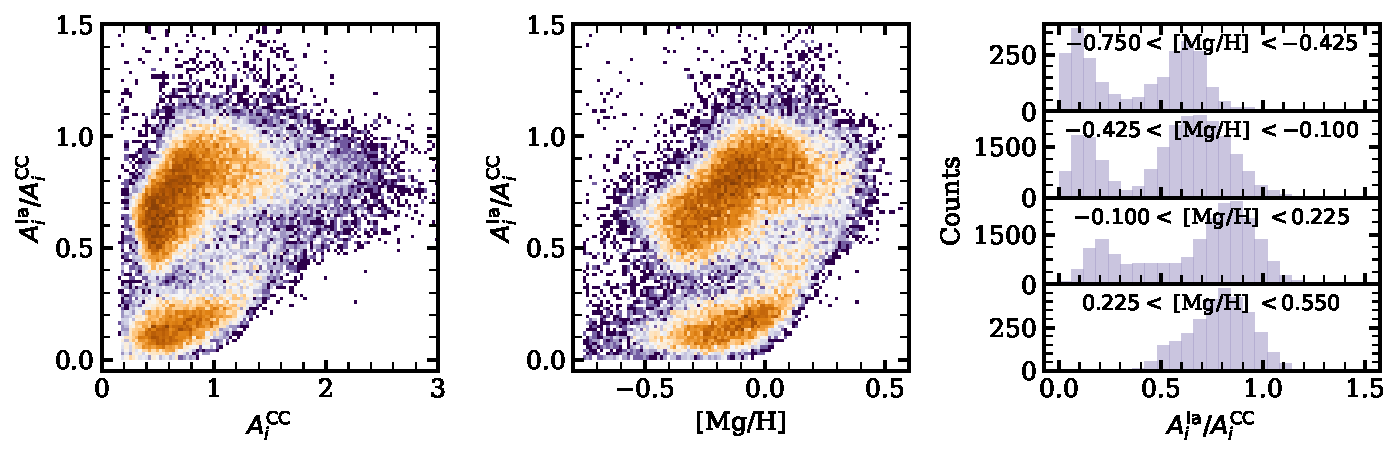
\includegraphics[width=.9\textwidth]{Paper/Figures/As.pdf}
    \caption{Left: distribution of $\AIa/\Acc$ vs. $\Acc$ for the fiducial model. Right: distribution of $\AIa/\Acc$ vs. $\mgh$. In both panels we can clearly see the bimodality to high values of $\Acc$ and $\mgh$.}
    \label{fig:As}
\end{figure*}

With the optimized process parameters in hand, we can use Equation~\ref{eq:xh} to calculate predicted abundances for the fiducial model---the abundances our stellar population would have if the model assumptions are correct and only one prompt and one delayed process contribute. To simulate observational noise, we add an error drawn from a Gaussian distribution with $\sigma$ equal to the reported error on each abundance for each star. In Figure~\ref{fig:all_param1} and~\ref{fig:all_param2} we plot the predicted abundances plus estimated noise in the second columns. These distributions can be compared the the observed abundance distribution in the first columns.

Overall, the fiducial model successfully reproduces the observed abundance distributions. It is capable of capturing metalicity dependences and bimodality. The predicted abundances plus estimated noise are not, however, able to reproduce the observed abundance scatter. This is especially noticeable at low-metallicity for C+N, Na, Al, K, Co, and Ce. For these elements the scatter in the observed abundance distribution is much larger than in the predicted distribution, suggesting that either the $K=2$ model is insufficient or that the APOGEE scatter is underestimated.

\subsection{Comparing to W22}\label{subsec:w22}

As discussed in Sections~\ref{sec:intro} and~\ref{sec:model}, \name{} is based upon the two-process model developed in W19 and W22, but with increased flexibility and no forced dependence upon the [Fe/Mg] vs. [Fe/H] bimodality or population abundance trends. Further, the \name{} utilizes all stellar abundances in the optimization of $\Acc$ and $\AIa$, where as only Mg and Fe are used in W19 and only Mg, O, Si, Ca, Fe, and Ni in W22. 

In the fiducial model, we adopt $K=2$, as in W22, but assume $\qccFe = 0.4$, 0.1 dex lower than the $\qccFe$ value assumed in W22. In practice, this moves the implied ``pure'' CCSN enrichment plateau from $\femg=-0.3$ to $\femg=-0.4$ (though the W22 plateau value is determined \textit{after} they apply a global offset of +0.05 to all $\femg$ abundances). Because our model is non-negative, it requires a lower $\qccFe$ to correctly model the stars on the $\femg$ plateau, where as W22 assigns stars with $\femg < -0.3$ negative $\AIa$ values.

While our stellar samples and model assumptions differ, we plot the W22 $\qcc$ and $\qIa$ vector components as well as the W22 solar metallicity $\fcc$ values in of Figures~\ref{fig:all_param1} and~\ref{fig:all_param2} for comparison with our fiducial model. We generally observe similar behavior between \name{} and W22. Our $\qIa$ vector components tend to be $\sim 0.1$ greater than those of W22 for elements with significant delayed contributions because of our differing $\qccFe$ assumptions. The metallicity dependencies agree for most elements, with small variations at the high-$\mgh$ end for O, Al, K, and Ce. We also see good agreement between the \name{} and W22 solar metallicity $\fcc$ values, with the W22 points slightly offset to larger values for elements with significant delayed contributions.

To compare the accuracy of the models' abilities to reproduce the observed abundances, we identify a subset of $\sim 23,000$ stars in both our sample and the W22 sample. We calculate the predicted abundances for each star under \name{} and the two-process model, then determine the $\chi^2$ value of the fits for each star (summing over the elements) and for each element (summing over the stars). We plot the cumulative stellar $\log(\chi^2)$ distribution and the total $\chi^2$ for each element in the right and left panels, respectively, of Figure~\ref{fig:comp_w22}. It is important to note that in the calculation of the W22 model residuals, we do not apply the temperature corrections discussed in Section 5.1 of W22. We find that, overall, the $\log(\chi^2)$ decreases between the W22 two-process model and our $K$-process model, an indication that we better predict the stellar abundances. When looking at each element individually, we find that we better predict C+N, Na, K, Ni, Mn, Co, and Ce, with major improvements to C+N and Mn. Our fiducial model is significantly worse at predicting Mg, Ca, and Fe than the W22 model, three of the six elements that W22 employ to fit the process amplitudes. Because \name{} uses all elements in its optimization, Mg, Ca, and Fe are effectively de-weighted relative to the W22 model, while C+N and Mn influence the model parameters.

\begin{figure*}[htb!]
    \centering
    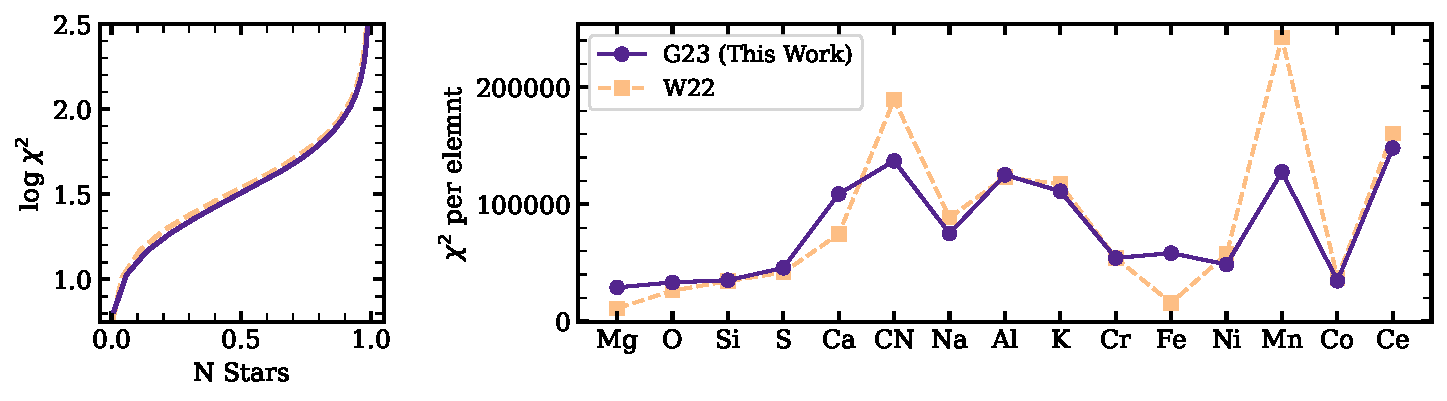
\includegraphics[width=\textwidth]{Paper/Figures/comp_w22.pdf}
    \caption{Left: cumulative distribution of $\log \chi^2$ for W22 (dashed orange line) and our fiducial model (G23, solid purple line). Right: $\chi^2$ per element for the same model fits. }
    \label{fig:comp_w22}
\end{figure*}

We note that our fiducial model is fit to a stellar sample that spans a wider range of $\teff$ and $\logg$ than the W22 sample. If we repeat our analysis on the W22 stellar sample with $\qccFe=0.5$ we almost perfectly recover the W22 process vector components, with small deviations at $\mgh>0.1$, and more substantially improve upon the stellar and elemental $\chi^2$ values. Most notably, \name{} is better able to predict the abundances of stars with $\mgh>0$, where the high-Ia and low-Ia sequences blend together and the W22 categorization of high-Ia and low-Ia stars may be incorrect.

\section{Variations Away from the Fiducial Model} \label{sec:variations}

\subsection{Choice of $\qccFe$} \label{subsec:qccFe}

While \name{} is flexible, we still include some quantitative assumptions, which we make to break exact model degeneracies (see Section~\ref{sec:model}).
Specifically, for each process, we choose one element to assign a ``known'' process vector element at all metallicities.
These are Mg and Fe in the 2-process case.
Specifically, for the prompt process, we ground our assumption in the nucleosynthetic theory that Mg is a pure CCSN element \citep[e.g.,][]{andrews2017}.
Unfortunately there is no comparable pure SNIa element, nor is there an element for which we know the relative CCSN/SNIa ratio.
In order to break an exact degeneracy between the prompt and delayed processes, we choose to fix the Fe process vector components, making unsubstantiated assumptions about Fe enrichment.

In the fiducial model, we choose $\qccFe = 0.4$ as this parameter choice is able to reproduce the observed [Fe/Mg] vs. [Mg/H] abundance distribution, as discussed in Section~\ref{subsec:parameters}. This choice impacts the predicted abundances as well as the implied $\fcc$ values of each star. Because our model is non-negative, the choice of $\qccFe$ sets the minimum [Fe/Mg] value attainable by our model ($\log_{10}(\qccFe)$). In this section, we explore the implications of different $\qccFe$ assumptions, varying the zero point and metallicity dependence ($\dqccFe$). In Figure~\ref{fig:qccFe_FeMg}, we plot the minimum [Fe/Mg] as a function of $\mgh$ for the $\qccFe$ and $\dqccFe$ parameters we explore. With a $\dqccFe=0.0$, we choose $\qccFe=0.5$ (the W22 value), 0.45 (approximate plateau value at $\mgh=-0.75$), 0.4 (the fiducial value that skirts the edge of the distribution), and 0.35 (captures almost all stars). With a $\dqccFe=0.15$, which roughly matches the slope of the low-Ia sequence at intermediate metallicity, we choose $\qccFe=0.5$ (passes through the center of the low-Ia density), 0.4 (skirts the edge of the distribution), and 0.35 (captures almost all stars).

\begin{figure*}[htb!]
    \centering
    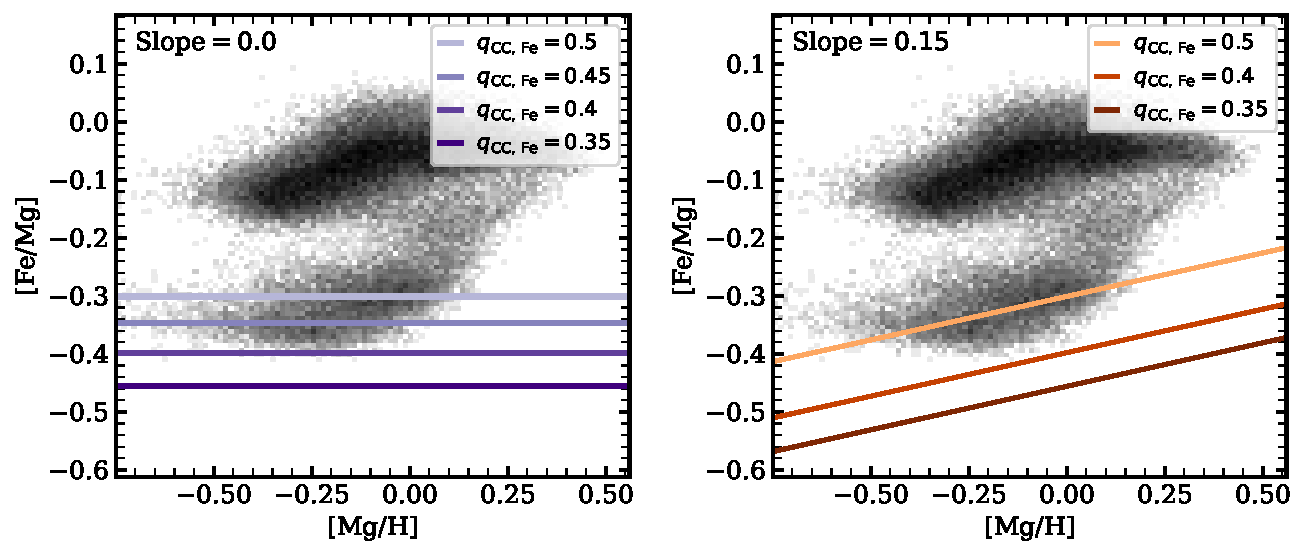
\includegraphics[width=\textwidth]{Paper/Figures/qccFe_FeMg.pdf}
    \caption{Minimum [Fe/Mg] value attainable for $\qccFe$ and $\dqccFe$ assumptions. Left: For $\dqccFe=0$ with $\qccFe=0.5$, 0.45, 0.4, and 0.35 (light to dark purple). Right: For $\dqccFe=0.15$ with $\qccFe=0.5$, 0.4, 0.35 (light to dark orange).}
    \label{fig:qccFe_FeMg}
\end{figure*}

We repeat the optimization of the \name{} with $K=2$ and these $\qccFe$ assumptions. In Figure~\ref{fig:qccFe_FeMgpred}, we plot the resulting predicted abundance distributions plus estimated noise. We do not plot the prediction for the fiducial model ($\qccFe=0.4$, $\dqccFe=0.0$), as this is shown in Figure~\ref{fig:all_param2}. Both models with $\qccFe=0.5$ fail to reproduce the shape and width of the low-Ia abundance distribution. They instead predict a much thinner sequence that is flat for $\dqccFe=0.0$ or slightly inclined for $\dqccFe=0.15$. The model with $\qccFe=0.45$ and $\dqccFe=0.0$ is better, but still predicts a low-Ia abundance distribution that is too thin, flat, and dense. The other four models ($\qccFe=0.35$ and $\qccFe=0.4$ with $\dqccFe=0.0$ and $\dqccFe=0.15$) predict an abundance distribution that strongly resembles the observed. There are minor differences in the low [Fe/Mg] and low [Mg/H] region, but it is difficult to tell by eye which model is best.

\begin{figure*}[htb!]
    \centering
    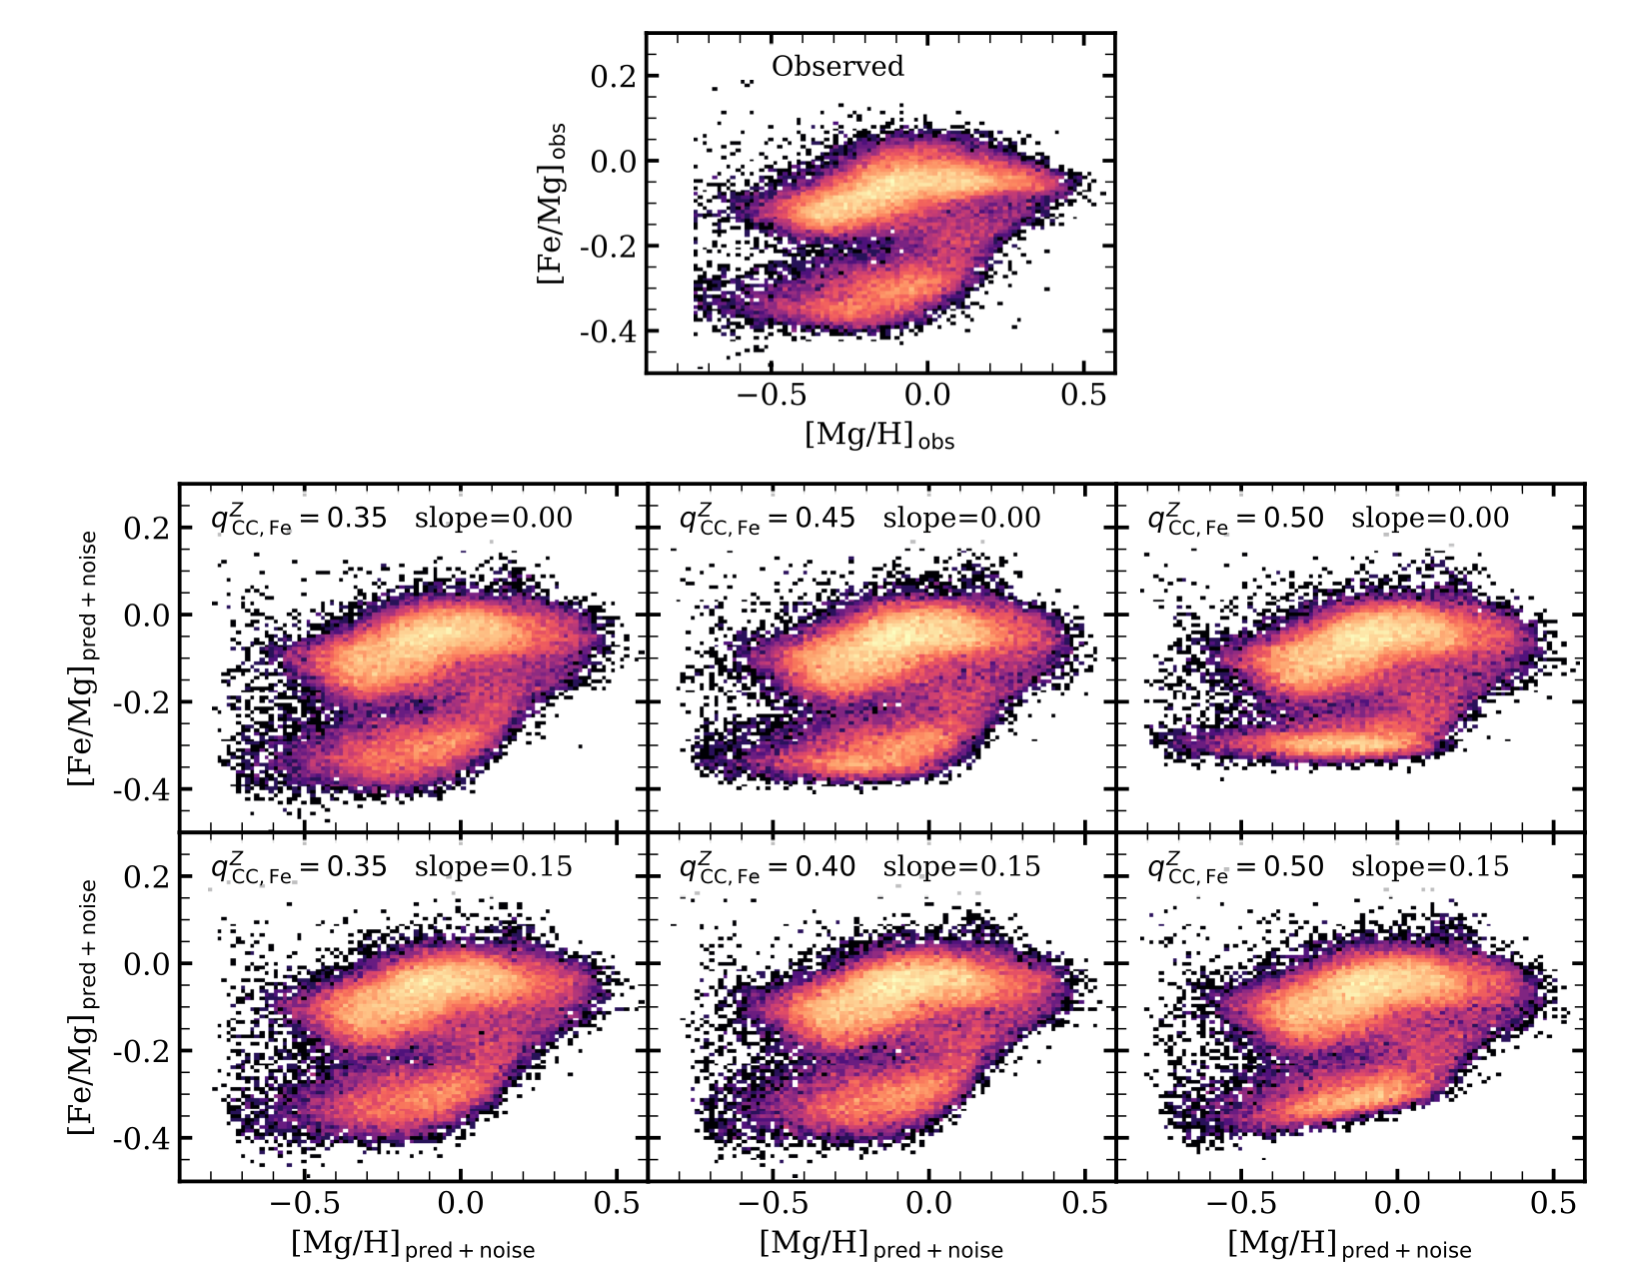
\includegraphics[width=\textwidth]{Paper/Figures/qccFe_FeMgpred.pdf}
    \caption{Predicted [Fe/Mg] vs. [Mg/H] abundance distributions plus estimated noise for models with $\dqccFe=0.0$ (top row) and $\dqccFe=0.15$ (bottom row). The $\qccFe$ value increase from left to right from 0.35 to 0.5. $\qccFe$ and $\dqccFe$ parameters are listed in each panel.}
    \label{fig:qccFe_FeMgpred}
\end{figure*}

To better assess the goodness of fit of each model, we calculate the average $\chi^2$ value per star. The models with $\qccFe$ of 0.5 and 0.45, regardless of $\dqccFe$, have an average $\chi^2$ per star $>90$ while the models with $\qccFe$ of 0.4 and 0.35 have an average $\chi^2$ per star $< 55$. In both the metallicity independent and metalicity dependent cases, the models with $\qccFe=0.4$ have the lowest average $\chi^2$ per star, at 54.54 and 54.47, respectively, though the models with $\qccFe=0.35$ have a $\chi^2$ that is only greater by $\sim0.1$. Of the seven models explored here, the case with $\qccFe=0.4$ and $\dqccFe=0.15$ has the lowest average $\chi^2$ per star, indicating that the Fe abundances are best fit by a metallicity dependent prompt process. 

Though the $\qccFe= 0.4$ and 0.35 models are similar in terms of their goodness of fit, their nucleosynthesis implications are more significant. In Figure~\ref{fig:qccFe_fcc}, we plot the median value of $\fcc$ (Equation~\ref{eq:fcc}) for the low-Ia population at solar metallicity ($-0.05 < \mgh < 0.05$), where low-Ia stars are defined by
\begin{equation}\label{eq:lowIa}
\begin{cases}
\mgfe > 0.12 - 0.13 \, \feh,    & \feh<0 \cr
\mgfe > 0.12,               & \feh>0, \cr
\end{cases}
\end{equation}
as in W19, W22, and G22.
We only show the median $\fcc$ values for the models with $\dqccFe=0.0$ as the solar metallicity median $\fcc$ values for the metallicity dependent models are almost identical for matching values of $\qccFe$. We find that the choice of $\qccFe$ has little impact on the median $\fcc$ values of elements dominated by CCSN enrichment (e.g. O, S, Al, K). As the delayed contribution increases, the median elemental $\fcc$ values decrease more significantly with decreasing $\qccFe$. The choice of $\qccFe$ most impacts the median $\fcc$ values for Na, Cr, Fe, Mn, and Ce, with the median $\fcc$ for Mn decreasing from 0.42 for $\qccFe=0.5$ to 0.22 for $\qccFe=0.35$. Because the $\qccFe$ value sets the prompt enrichment plateau, a lower $\qccFe$ model implies a lower $\fcc$ value. 

While the high $\qccFe$ model can likely be ruled out due to poorness of fit, the true $\qccFe$ value and its metallicity dependence are unknown. It is therefore important not to over-interpret the specific $\fcc$ values of a given model. The $\fcc$ parameter can provide qualitative descriptions of which elements have more or less prompt/delayed enrichment, but the exact values are uncertain.

\begin{figure*}[htb!]
    \centering
    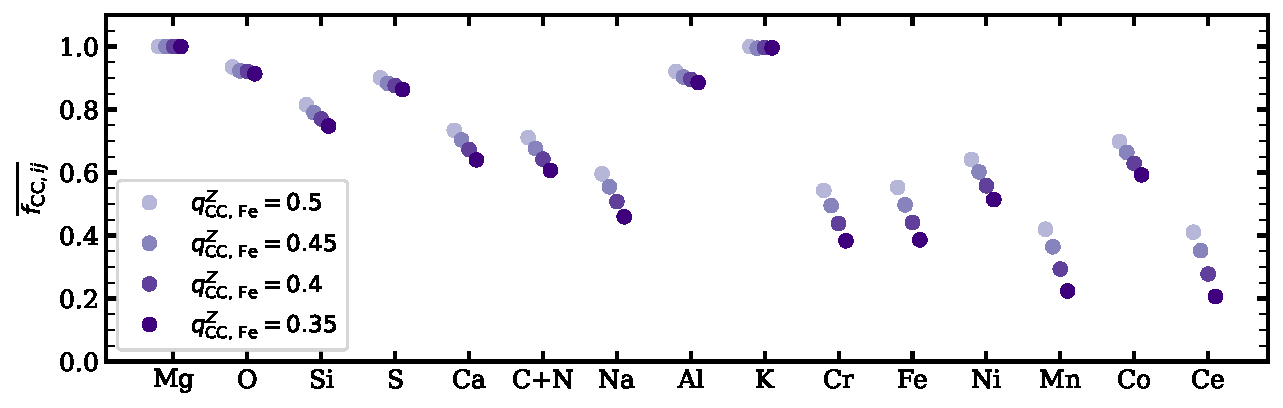
\includegraphics[width=\textwidth]{Paper/Figures/qccFe_fcc.pdf}
    \caption{Elemental median values of $\fcc$ at solar metallicity for the low-Ia population for \name{} with $\qccFe=0.35$ (darkest purple) to 0.5 (lightest purple) and $\dqccFe=0.0$.}
    \label{fig:qccFe_fcc}
\end{figure*}

\subsection{Increasing the Number of Processes} \label{subsec:k=4}

In our fiducial model, we adopt $K=2$ with the two processes representing prompt, CCSN-like enrichment and delayed, SNIa-like enrichment. While a $K=2$ model can well describe the stellar abundances (e.g., Figures~\ref{fig:all_param1} and~\ref{fig:all_param2}), the abundance residuals cannot be explained by observational noise alone and hold information about the intrinsic variations from a $K=2$ model (G22, W22, \citealp{ting2022}). Potential sources of such scatter include metallicity-dependent SN yields with a bursty star formation history, environmental variations in the IMF, stochastic sampling of the IMF, and more than two distinct processes (e.g., AGB stars, merging neutron stars, and unique classes of SNIa) with different time delays for enrichment \citep[e.g.][]{belokurov2022, griffith2023}. 

In this section, we will explore the impact of adding additional processes to our model, increasing from $K=2$ to $K=4$. Our goal is to demonstrate the potential of using \name{} to capture more of the observed abundance diversity. Because \name{} is sensitive to enrichment with different time delays, adding components could be interpreted as adding sources with distinct enrichment time scales. For example, if AGB stars and SNIa enrich with the \textit{same} time delay, the model would fit both sources in one delayed component. If AGB and SNIa enrich with \textit{different} delay times, a third component should pick up delayed AGB enrichment not captured by the original delayed process. Indeed, evidence of a distinct AGB-like process is identified in G22 and W22, where correlated residuals are used to expand the two-process model. However, both works add components in a restrictive manner that requires choosing which elements to assign to 3rd and/or 4th processes and that does not allow for the original two processes to vary. 

We take a more flexible approach, allowing the model to identify the elements best-fit with additional components and modify the $K=2$ process parameters. Ultimately, such a method could be used to identify elements with more than two enrichment channels, but we will refrain from over-interpretation here. Our model now includes four components, such that
\begin{equation}\label{eq:mij_4}
    m_{ij} = \log_{10}(\Acc\,\qcc + \AIa\,\qIa + A_{i}^{3}\,q_{3, j}^{Z} + A_{i}^{4}\,q_{4, j}^{Z}),
\end{equation}
where $q_{3, j}^{Z}$ and $q_{4, j}^{Z}$ are the third and fourth process vector components and $ A_{i}^3$ and $A_{i}^4$ are the third and fourth process amplitudes. The model, however, does require some regularization to converge. As in the $K=2$ case where we assume that Mg is a pure CCSN element and fix the $\qccFe$ and $\qIaFe$ values, we need elements to regulate of our 3rd and 4th processes. We choose Ce and Mn, two elements with larger residuals that likely have additional nucleosynthetic sources---Ce from AGB stars and Mn from unique classes of SNIa \citep[e.g.][]{gallino1998, reyes2020, gronow2021}. We initialize the $K=4$ model at the $K=2$ model values of $\qcc$, $\qIa$, $\Acc$, and $\AIa$ with the added constraints that 
\begin{equation}\label{eq:q3_z}
    q_{{\rm 3, Mg}}^{\,Z} = 0, \quad 
    q_{{\rm 3, Fe}}^{\,Z} = 0,  \quad 
    q_{{\rm 3, Mn}}^{\,Z} = 0, \quad 
    q_{{\rm 3, Ce}}^{\,Z} = 1 \quad 
\end{equation}
and 
\begin{equation}\label{eq:q4_z}
    q_{{\rm 4, Mg}}^{\,Z} = 0, \quad 
    q_{{\rm 4, Fe}}^{\,Z} = 0,  \quad 
    q_{{\rm 4, Mn}}^{\,Z} = 1, \quad 
    q_{{\rm 4, Ce}}^{\,Z} = 0. \quad 
\end{equation}
We first fit the $A$-step to only Mg, Fe, Mn, and Ce, and then conduct 32 iterations of the $q$-step and $A$-step, as described in Section~\ref{sec:model}. We again inflate the according to Equation~\ref{eq:inflate_ivar} with $Q=5$. 

The model converges upon a set of process vector components and amplitudes that can be combined with Equation~\ref{eq:mij_4} to predict the stellar abundances and calculate the fractional contribution from each process. The model parameters themselves are less directly interpretable, as we set the third and fourth process vector components for Ce and Mn to an arbitrary value with no metallicity dependence, so we do not show them here. We calculate $\fcc$, $f_{{\rm Ia}, ij}$, $f_{3, ij}$, and $f_{4, ij}$ for each abundance of each star where
\begin{equation}\label{eq:fX}
    f_{k, ij} = \frac{A_{i}^{k} \, q_{k,j}^Z}{\Acc\,\qcc + \AIa\,\qIa + A_{i}^{3}\,q_{3, j}^{Z} + A_{i}^{4}\,q_{4, j}^{Z}}.
\end{equation}
We find that the third process, regularized to Ce, contributes minorly to O, Si, S, Al, and K and more significantly to Ca, Na, Cr, and Ce. The fourth process, regularized to Mn, contributes minorly to K and more significantly to S, C+N, Na, Cr, Ni, Mn, and Co. These best-fit element groupings resemble but are not identical to the elements selected for additional components in W22, where the third process included Ca, Na, Al, K, Cr, and Ce and the fourth process included Ni, V, Mn, and Co. 

In the fourth column of Figure~\ref{fig:all_paramK}, we plot the median $f_{K, ij}$ as a function of $\mgh$ of the low-Ia population (Equation~\ref{eq:lowIa}) for a subset of elements with significant contributions from the third and/or fourth processes. We include median $\fcc$ and $f_{{\rm Ia},ij}$ from the $K=2$ model for comparison. We see that the third process contributes significantly to Ca, Na, Cr, and Ce at low metallicity, with decreasing contribution up to $\mgh\approx0.1$. The fractional contribution from the $K=2$ prompt and delayed processes to these elements decreases under the $K=4$ model, with median $\fcc$ decreasing more substantially than $f_{{\rm Ia}, ij}$. The fourth process behaves in a similar manner but with elements C+N, Na, Cr, Ni, Mn, and Co. We find that the addition of a fourth process decreases $\fcc$ and $f_{\rm Ia}$ values by roughly equal amounts at low metallicities. The fractional contribution from the third and fourth process is nearly identical in the high-Ia population, though the median $\fcc$ and $f_{{\rm Ia}, ij}$ values vary more significantly (as seen in Figures~\ref{fig:all_param1} and~\ref{fig:all_param2}).

Adding model components increases the abundance diversity that \name{} can achieve. In the left-most columns of Figure~\ref{fig:all_paramK}, we plot the $\xmg$ v.s. $\mgh$ distributions for the observed stellar sample, the $K=2$ model predictions, and the $K=4$ model predictions for Ca, C+N, Na, Cr, Ni, Mn, Co, and Ce. We note that the predicted abundances do \textit{not} have noise added (unlike Figures~\ref{fig:all_param1} and~\ref{fig:all_param2}). Comparing the predicted abundances from the $K=2$ and $K=4$ process models, we see that the $K=4$ process model is better able to capture the observed abundance distribution than the $K=2$ model. Specifically, it better captures the scatter in the low metallicity end of the low-Ia population. 

\begin{figure*}[htb!]
    \centering
    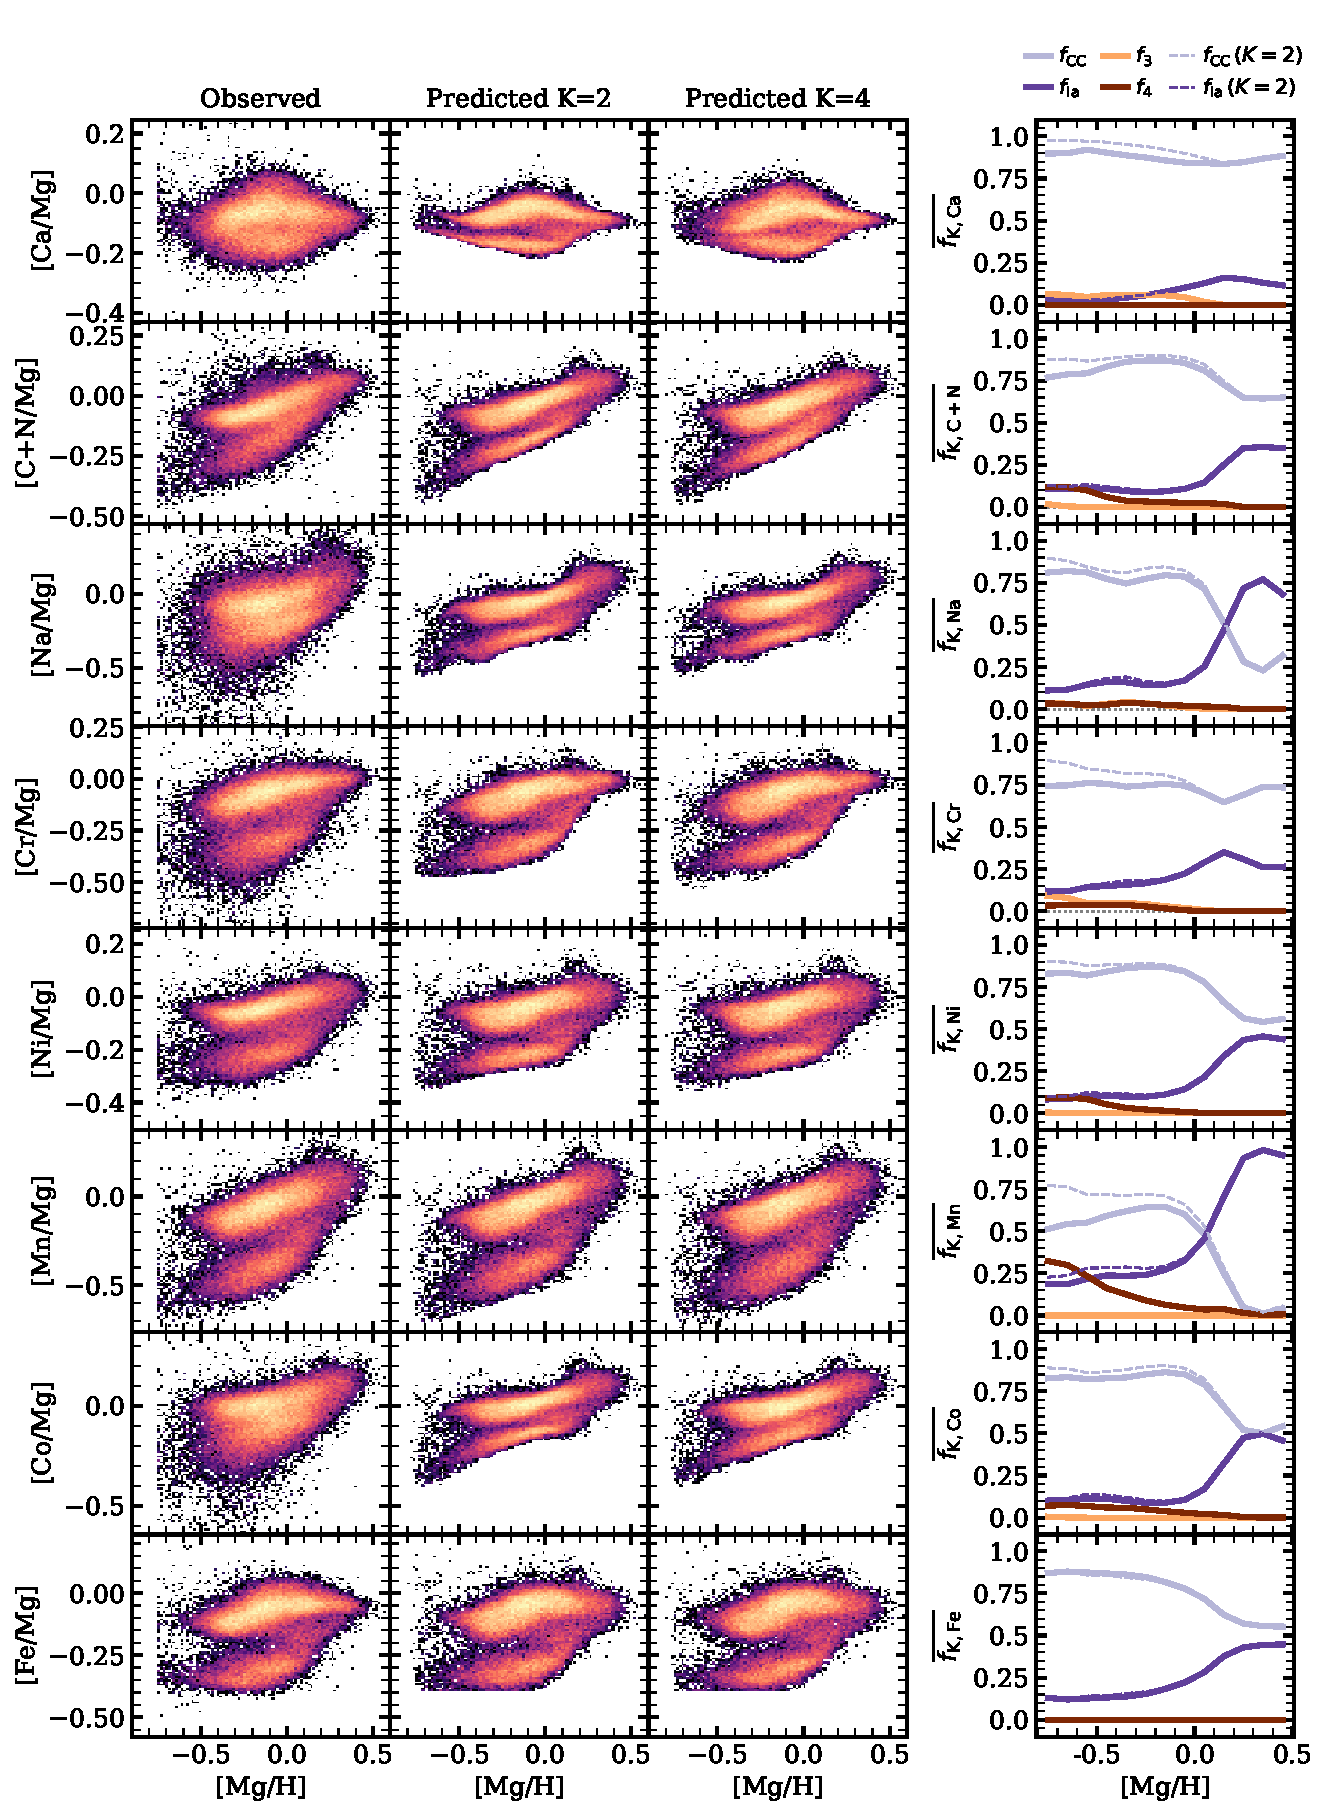
\includegraphics[width=\textwidth]{Paper/Figures/all_param_k4.pdf}
    \caption{Left: [X/Mg] vs. [Mg/H] abundance distributions for the observed sample (first column), $K=2$ model (second column) and $K=4$ model (third column) for Ca, C+N, Na, Cr, Ni, Mn, Co, and Ce. Right: median fractional contribution from each process for the $K=4$ (solid lines) and $K=2$ (dashed lines) models to the low-Ia population as a function of $\mgh$. We plot the median $\fcc$ in light purple, $f_{{\rm Ia}, ij}$ in dark purple, $f_{3, ij}$ in light orange, and $f_{4, ij}$ in dark orange as well as a dotted grey line at 0 for reference.} 
    \label{fig:all_paramK}
\end{figure*}

The improved ability of the $K=4$ model to capture the abundance diversity of our stellar sample is also clear in the fit statistics. In Figure~\ref{fig:comp_Ks}, we plot the cumulative $\log(\chi^2)$ distributions for the fits to each star and the total $\chi^2$ for each element for the fiducial $K=2$ model and the $K=4$ model. We see that the cumulative $\log(\chi^2)$ distribution decreases with the increase in model components. We also find that the $\chi^2$ per element is lower for all elements in the $K=4$ model. Significant improvements to Ca, C+N, Mn, and Ce are likely due to the additional third and fourth components capturing abundance patterns that the original prompt and delayed processes could not. Notably, we also see a significant improvement in the Fe fit, even though we require $q_{\rm 3,Fe}^{Z} = q_{\rm 4,Fe}^{Z} = 0$. Because all elements influence the $K=2$ model fit, the fiducial model was likely pulled away from the best solution for Fe to accommodate another element, like Mn. With the additional components able to account for the non-Fe-like enrichment, the original two processes are better able to capture the Fe enrichment. 

\begin{figure*}[htb!]
    \centering
    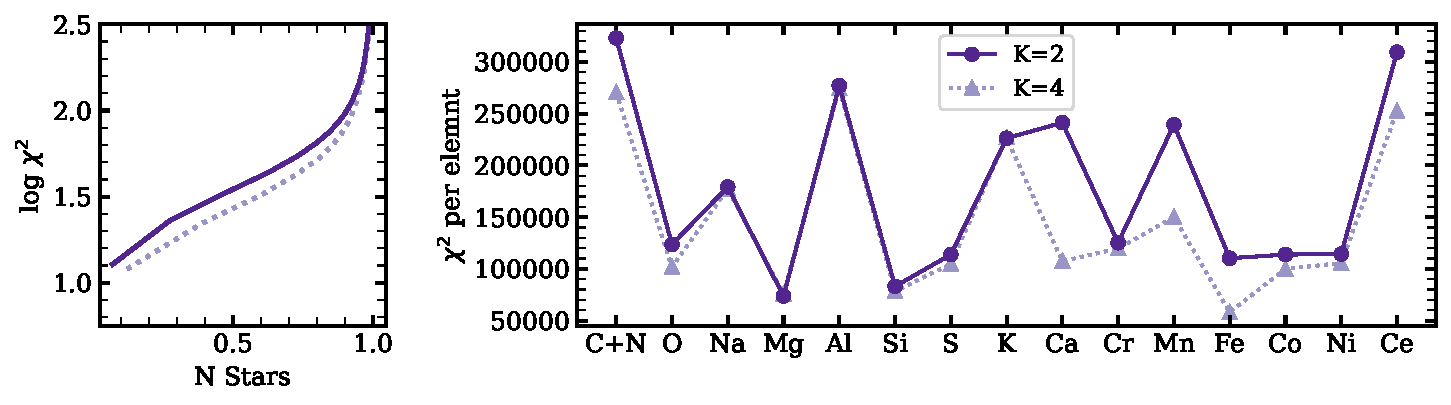
\includegraphics[width=\textwidth]{Paper/Figures/comp_Ks.pdf}
    \caption{Left: cumulative distribution of $\log \chi^2$ for the $K=2$ model (solid dark purple line) and our the $K=4$ model (dotted light purple line). Right: $\chi^2$ per element for the same model fits.}
    \label{fig:comp_Ks}
\end{figure*}

Through this investigation, we find that \name{} is extendable to $K>2$ processes. Adding components improves the model's ability to capture the observed abundance diversity. We will not interpret these results in terms of nucleosynthesis here, but provide a discussion of the future science that \name{} and the $K=4$ model enable below.

\section{Discussion}\label{sec:discussion}

In this paper, we present \name{}, a flexible and data-driven model of for nucleosynthesis. \name{} describes stellar abundances as the sum of $K$ components, where each component is the product of a metallicity-dependent process vector component (fit to each element) and a process amplitude (fit to each star).    Combined with a likelihood function and a set of assumptions (Section~\ref{sec:model}) that make the processes interpretable in terms of nucleosynthetic sources, the best-fit \name{} parameters can be used to calculate fractional contributions from each process as well as a full suite of predicted $K$ process abundances. 

We fit \name{} with $K=2$ to 15 abundances labels for 48,659 RGB stars in APOGEE DR17, selecting a population that minimizes statistical and systematic errors while spanning an [Mg/H] of -0.8 to 0.5. In the $K=2$ model, the first process, fixed to Mg, represents prompt CCSN-like enrichment, and the second process, fixed to Fe, represents delayed SNIa-like enrichment---but other nucleosynthetic sources with similar time delays may be mixed into each. Overall, we find that $K=2$ is a good fit to the data and that the model successfully recovers the global abundance patterns in the Milky Way. While \name{} does not rely on $\femg$ vs. $\mgh$ bimodality or median abundance trends, it is able to recover the observed bimodal abundance distribution. Further, the fit parameters $\Acc$ and $\AIa$ act as ``denoised'' abundance labels, and reveal a clearer signature of bimodality at high-metallicity in $\AIa/\Acc$ vs. $\mgh$ space than in $\femg$ vs. $\mgh$. This suggests that the \name{} fit parameters and predicted abundances could be used as a higher signal-to-noise tracer of nucleosynthesis, as they are condensing information from 15 elements into two variables. 

To test the assumptions of the fiducial model, we explore the impact of varying the fixed value of $\qccFe$. We find that high values of $\qccFe$ (0.5 and 0.45) are not able to reproduce the observed [Fe/Mg] vs [Mg/H] abundance distribution, regardless of the process vector component's metallicity dependence, and that values $\qccFe = 0.4$ and 0.35 with $\dqccFe = 0$ or 0.15 produces similarly successful fits. While predicted abundance distributions appear similar for these models, the implied fractional contribution from the prompt process is strongly dependent upon the Fe assumption for elements with substantial delayed enrichment. Through this exploration, we conclude that the quantitative nucleosynthetic interpretation of \name{} is dependent upon the input assumptions, and that there is inherent uncertainty in the $\fcc$ values. 

Finally, we expand \name{} from $K=2$ to $K=4$, regularizing the third and fourth processes to Ce and Mn. \name{} builds off of the original model, such that the $K=4$ model starts at the $K=2$ solution and then finds the best-fit parameters for $K=4$, altering the original solution and allowing all elements (except Mg and Fe) to have contributions from additional processes. We find that S, Ca, C+N, Na, Cr, Mn, Co, Ni, and Ce are best fit with a third and/or fourth component, with such processes contributing most significantly at low metallicity. The $K=4$ model improves the ability of \name{} to fit the abundances of all elements but especially improves predictions of Ca, C+N, Fe, Mn, and Ce. This successful implementation of a $K=4$ model shows that \name{} can be extended to $K>2$, and it has potential future use in constraining enrichment beyond a single prompt and delayed process---critical to understanding enrichment from AGB stars, merging neutron stars, and rarer novae.

\name{} is based upon the two-process model developed in W19 and W22. While the two models are identical in format for the $K=2$ case, the model assumptions, parameter derivations, and implementations differ. The W22 two-process model derives process vector components from median abundance trends, reliant upon $\mgfe$ vs. $\mgh$ bimodality, and fits process amplitudes to a subset of $2-6$ $\alpha$ and Fe-peak elements. \name{}, on the other hand, employs a likelihood function fit to all stars and all elements to derive both process amplitudes and vector components. Our more data-driven implementation results in the improved ability to predict stellar abundances. Notably, \name{} can better predict C+N and Mn abundances than the W22 two-process model, since all elements are used to constrain the fits. The most significant improvement to the original two-process model, though, is in \name{}'s flexibility. The flexible implementation of the model allows us to easily vary the assumptions, such as $\qccFe$, and increase the number of model components to study the impact of our assumptions on the results and push the interpretation of \name{} beyond standard CCSN and SNIa nucleosynthesis in a less restrictive manner than W22 and G22. 

However, \name{} is not without its own faults. The assumptions listed in Section~\ref{sec:model} may incorrectly skew our results and the model could benefit from improvements in implementation. While assumptions (4) and (5) on Mg and Fe production are flexible, \name{} requires that both elements have fixed process vector components. If our assumptions are incorrect and, for instance, Mg is not a pure prompt element or (in the $K=4$ case)  Fe has contributions from multiple delayed sources, our nucleosynthetic interpretation of \name{} may be incorrect. Additionally, assumption (7) states that the APOGEE data products can be used for this project, but that we inflate abundance errors with a softening parameter, $Q$ to account for their likely underestimation. If the APOGEE errors are correct, this assumption could pull the model away from a solution that favors true outlier points. In future \name{} implementation, the development of a more robust method to justifiably de-weighting outlier stars from the global fits would be beneficial. Finally, \name{} fits process vector components along a spline with 11 knots (assumption 6). As this method fits a polynomial between each knot, it can result in sharp features at the knot locations in metallicity regions with few points or large scatter. Fitting process vector components with a continuous function would be more ideal, though Appendix C.1 in G22 suggests that this change will have minimal impact on the results. 
\ejg{Hogg add a bit about expanding to a more general latent-variable model?}

Beyond improvements to the underlying model assumptions and implementation, \name{} needs to include parameter uncertainty. While the model delivers process vector components and amplitudes, which can be used to calculate $f_{K, ij}$ and $K$ process predicted abundances, the current implementation does not return errors on any variable. The best method to derive such errors has not been explored, but one could use the likelihood function or bootstrapping. These methods will encapsulate the uncertainty on process parameters from the APOGEE abundance errors but will not capture the uncertainty due to model assumptions, such as $\qccFe$ (Section~\ref{subsec:qccFe}). 

While such future changes will improve the model, the current form of \name{} and its data products can support ongoing research and will enable new science. Most immediately, \name{} provides high signal-to-noise abundance labels, $\Acc$ and $\AIa$, as well as de-noised stellar abundances ($m_{ij}$). $\Acc$ and $\AIa$, in particular, are powerful tracers of nucleosynthesis. \ejg{Hogg add a bit about overall $\alpha$/M indicators.} In Section~\ref{subsec:parameters}, we showed that the high-Ia and low-Ia populations are more clearly defined in $\AIa/\Acc$ vs. [Mg/H] than in [Fe/Mg] vs/ [Mg/H]. In amplitude space, the low-Ia population can be re-defined as 
\begin{equation}\label{eq:lowIa new}
\begin{cases}
\AIa/\Acc < 0.35 ,    & \mgh<-0.2 \cr
\AIa/\Acc < 0.5 + 0.7 \, \mgh,  & -0.2\geq\mgh<0.1, \cr
\AIa/\Acc < 0.57 ,    & \mgh\geq0.1 \,. \cr
\end{cases}
\end{equation}
Compared to Equation~\ref{eq:lowIa} (W19, W22), this new definition re-classifies 647 stars as high-Ia and 224 stars as low-Ia. We show the location of these stars in $\AIa/\Acc$ vs. [Mg/H] and [Mg/Fe] vs. [Fe/H] in Figure~\ref{fig:pop_divis}. Many of the re-classified stars are at $\feh>-0.1$. When dividing in [Mg/Fe], it is difficult to correctly separate the populations at high metallicity, as they are blended together. Our new definition also re-classifies many stars near [Fe/H] of -0.3 as high-Ia, suggesting that the W19 and W22 high-Ia definition has too shallow a slope. While only $\sim 2\%$ of stars are re-classified under the new definition, we suggest that Equation~\ref{eq:lowIa new} be used to chemically define the low-Ia and high-Ia populations if \name{} fits are available, especially if studying stars with $\feh > -0.1$. 
Beyond improving the definition of high-Ia and low-Ia populations, the \name{} parameters and predicted abundances could be used in any current analysis that strives to show trends with abundance labels. We predict that trends of stellar parameters with [X/H] will be clearer when comparing to $[\text{X}/\text{H}]_{\rm pred}$, $\Acc$, or $\AIa$.

\begin{figure*}[htb!]
    \centering
    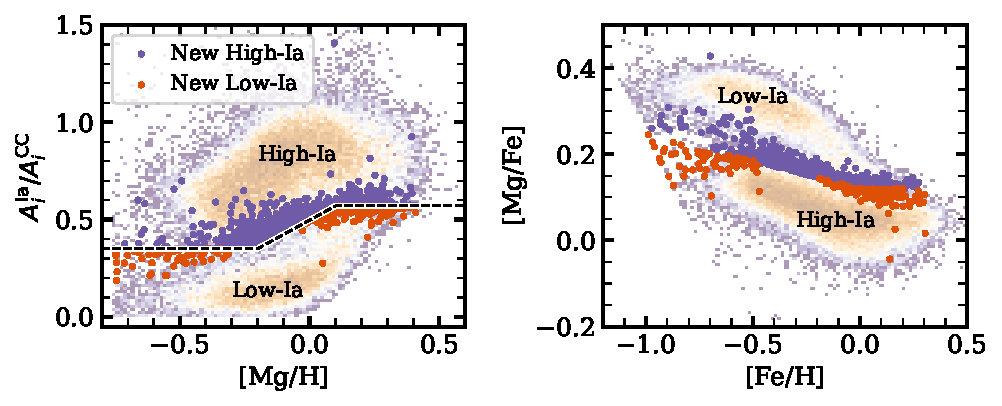
\includegraphics[width=.9\textwidth]{Paper/Figures/pop_divis.pdf}
    \caption{Left: distribution of stars in $\AIa/\Acc$ vs. [Mg/H] where the black dashed line is the dividing line between the high-Ia and low-Ia populations (Equation~\ref{eq:lowIa new}). Stars that are re-classified as high-Ia are shown in purple (647 stars) and stars that are re-classified as low-Ia are shown in orange (224 stars). Right: Same as left, but in [Mg/Fe] vs. [Fe/H] space. The high-Ia and low-Ia populations have been labeled in both panels for clarity.
    \label{fig:pop_divis}}
\end{figure*}

Such analysis with \name{} parameters will be useful in studying nucleosynthesis, dynamics, disk formation, stellar ages, and much more. However, in this paper we only present fits for a small population with restricted stellar parameters, relative to the full APOGEE sample. 
\ejg{Add some discussion about the data products that are available for the sample in this paper and the availability of our code....} While \name{} could be fit to the full APOGEE sample, systematic abundance effects with $\teff$ and $\logg$, as well as other abundance artifacts \citep[e.g.,][]{jonsson2020, griffith2021a}, cause the abundance trends to differ across the Hertzsprung-Russell diagram. The best-fit \name{} parameters for the giants would differ from those for the dwarfs. If such systematics could be accounted for (see Sit et al. in prep) we could fit the full APOGEE stellar sample with \name{}, or train \name{} on a subset of high signal-to-noise stars and apply the fits to the full sample. This potential future analysis could reveal additional information about the nucleosynthetic history of our Galaxy and would provide higher signal-to-noise abundance labels for the full sample.

The success of the two-process model (W19, W22) and \name{} with $K=2$ suggests that the disk is largely two-dimensional (2D). In this paper, we have focused on a 2D nucleosynetheic model, with the two dimensions representing prompt CCSN-like enrichment and delayed SNIa-like enrichment. However, another 2D class of theoretical models for the Milky Way exist, describing stars in terms of birth radius and birth date \citep[e.g.,][]{frankel2018, ness2022}. Are these two 2D models related? If they are, then the nucleosynthetic parameters from \name{} ($\AIa$ and $\Acc$) should predict asteroseismic ages (or masses), up to unpredictable aspects of mass transfer, as well as the guiding radius, up to unpredictable aspects of radial migration. While a deeper study of the implications of the disk's two-dimensionality is outside the scope of this work, we show the relationship between age and process amplitudes in Figure~\ref{fig:age}. Here we see a clear gradient in age with $\Acc$ and $\AIa/\Acc$ (as in G22 and W22), though outlier stars are scattered throughout. We predict that the \name{} parameters will be better age diagnostics than APOGEE abundances, and that age outliers may be mass transfer objects. 

\begin{figure*}[htb!]
    \centering
    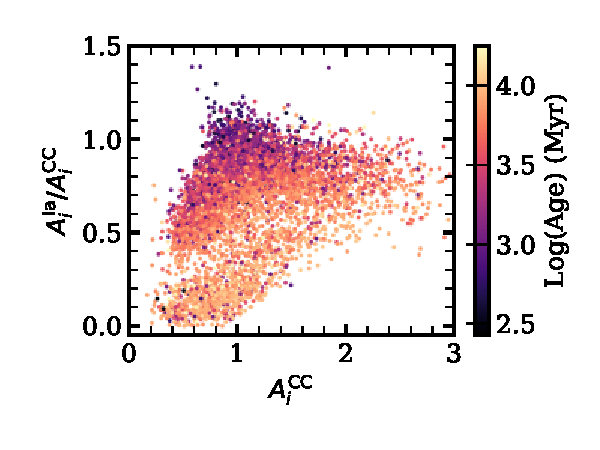
\includegraphics[width=.6\textwidth]{Paper/Figures/AIaAcc_age.pdf}
    \caption{$\AIa/\Acc$ vs. $\Acc$ distribution for stars in the APOKASC sample. Each point is colored by the star's log(Age), with younger stars in black and older stars in yellow.
    \label{fig:age}}
\end{figure*}

Finally, because of the flexibility of \name{}, new scientific applications are enabled that were not feasible before. Because \name{} does not rely on [Mg/Fe] vs. [Fe/H] bimodality, non-bimodal population can now be fit with a multi-component nucleosynthetic model. \name{} could be applied to the low metallicity disk, halo, Gaia Enceladus Sausage, Nebula Majora, Nebula Minora\footnote{Historically referred to as the LMC and SMC.}, other Milky Way satellites, and more. \name{} can also be easily extended to $K>2$ in a much less restricted way than the two-process model. While a $K=2$ model well describes the global abundance patterns, intrinsic residual scatter on the scale of 0.01 to 0.02 dex remains (\citealp{ting2022}, W22, G22). This scatter could be signatures of enrichment from non-CCSN/SNIa sources, stochastic sampling of the IMF, environmental IMF variations, or metallicity-dependent SN yields with a bursty star formation history \citep[e.g.][]{belokurov2022, griffith2023}. While it is difficult to identify non-CCSN or SNIa enrichment in the APOGEE data alone, where only C+N and Ce are likely to have significant contributions from other sources, there may be signatures in other surveys with better coverage of heavier elements. Applying a $K>2$ model to GALAH \citep{buder2021}, or an overlapping sample of APOGEE and GALAH stars \citep{nandakumar2022}, could prove more successful.

\ejg{Some concluding statement about the tons of future science that \name{} can do and how readers can access it.}

\section{Acknowledgements}
It is a pleasure to thank
  Melissa Ness (Columbia),
  Adrian Price-Whelan (Flatiron),
  Tawny Sit (OSU),
  Soledad Villar (JHU),
  David Weinberg (OSU),
  CU Boulder Research Computing services and staff,
  and the Astronomical Data group at the Flatiron Institute
for valuable discussions and help.
E.J.G. is supported by an NSF Astronomy and Astrophysics Postdoctoral Fellowship under award AST-2202135.

Funding for the Sloan Digital Sky Survey V has been provided by the Alfred P. Sloan Foundation, the Heising-Simons Foundation, the National Science Foundation, and the Participating Institutions. SDSS acknowledges support and resources from the Center for High-Performance Computing at the University of Utah. The SDSS web site is \url{www.sdss.org}.

SDSS is managed by the Astrophysical Research Consortium for the Participating Institutions of the SDSS Collaboration, including the Carnegie Institution for Science, Chilean National Time Allocation Committee (CNTAC) ratified researchers, the Gotham Participation Group, Harvard University, Heidelberg University, The Johns Hopkins University, L’Ecole polytechnique f\'{e}d\'{e}rale de Lausanne (EPFL), Leibniz-Institut f{\"u}r Astrophysik Potsdam (AIP), Max-Planck-Institut f{\"u}r Astronomie (MPIA Heidelberg), Max-Planck-Institut f{\"u}r Extraterrestrische Physik (MPE), Nanjing University, National Astronomical Observatories of China (NAOC), New Mexico State University, The Ohio State University, Pennsylvania State University, Smithsonian Astrophysical Observatory, Space Telescope Science Institute (STScI), the Stellar Astrophysics Participation Group, Universidad Nacional Aut\'{o}noma de M\'{e}xico, University of Arizona, University of Colorado Boulder, University of Illinois at Urbana-Champaign, University of Toronto, University of Utah, University of Virginia, Yale University, and Yunnan University.


\software{matplotlib \citep{hunter2007}, NumPy \citep{harris2020}, pandas \citep{pandasa, pandasb}, astropy \citep{astropy2013, astropy2018, astropy2022}, and jax \citep{jax}.}

\facilities{Sloan, Kepler}

\bibliography{sample631}{}
\bibliographystyle{aasjournal}

\end{document}

